%% ViACaPu — Bài báo IEEE (bản tiếng Việt, IEEEtran)
%% Biên dịch: pdflatex paper_ieee_vi.tex (2 lần để cập nhật tham chiếu)
%% Cần gói tiếng Việt. Trên Overleaf chọn compiler pdfLaTeX; nếu lỗi font,
%% đổi sang XeLaTeX và thay phần font ở dưới (xem ghi chú).
%% Ảnh: đặt thư mục figures/ cùng cấp với file .tex này.
\documentclass[conference,onecolumn]{IEEEtran}
\IEEEoverridecommandlockouts

\usepackage[utf8]{vietnam}   % hỗ trợ tiếng Việt (pdfLaTeX). Nếu không có, xem ghi chú cuối file.
\usepackage{cite}
\usepackage{amsmath,amssymb,amsfonts}
\usepackage{graphicx}
\usepackage{textcomp}
\usepackage{booktabs}
\usepackage{multirow}
\usepackage[margin=2.5cm]{geometry}   % lề cho bản 1 cột

\begin{document}

\title{ViACaPu: Mô Hình Nhẹ Nhận Biết Ngữ Âm cho\\
Khôi Phục Dấu Câu và Viết Hoa trong ASR Trên Thiết Bị}

\author{\IEEEauthorblockN{Nguyen Doan Sy, Ngoc Mai Xuan}
\IEEEauthorblockA{\textit{Hanoi University of Science and Technology}\\
Ha Noi, Vietnam}
}

\maketitle

\begin{abstract}
Khôi phục dấu câu và viết hoa giúp cải thiện khả năng đọc hiểu của văn bản nhận
dạng tiếng nói, nhưng các phương pháp dựa trên bộ mã hóa tiền huấn luyện lớn đòi
hỏi nhiều tài nguyên, còn các phương pháp tích hợp trực tiếp vào mô hình nhận dạng
hạn chế khả năng triển khai như một thành phần độc lập. Bài báo đề xuất ViACaPu,
một mô hình nhẹ 3,58 triệu tham số kết hợp thông tin âm học và văn bản để khôi
phục đồng thời dấu câu và viết hoa tiếng Việt, hoạt động như mô-đun hậu xử lý cho
hệ thống nhận dạng có sẵn mà không cần huấn luyện lại bộ nhận dạng. Mô hình dùng
cơ chế chú ý chéo có cổng: mỗi trạng thái cấp từ truy vấn trực tiếp chuỗi khung
log-Mel, nên không cần dấu thời gian mức từ. Đánh giá trên tập kiểm định tách từ
Dolly-1000h, với đầu vào là \emph{bản ghi tham chiếu} đã hạ chữ thường và loại bỏ
dấu câu (tức điều kiện $\mathrm{WER}=0$, đo năng lực khôi phục định dạng tách biệt
khỏi lỗi nhận dạng), ViACaPu nâng micro-F1 dấu câu từ $0{,}820$ lên $0{,}927$ và
micro-F1 viết hoa từ $0{,}937$ lên $0{,}944$ so với biến thể chỉ dùng văn bản cùng
kiến trúc, nhất quán qua ba seed, với 0,91 triệu tham số bổ sung. Mức cải thiện
tập trung ở dấu phẩy ($0{,}660 \rightarrow 0{,}888$), phù hợp với giả thuyết rằng
ranh giới mệnh đề gắn với khoảng lặng khi nói. Một lưới thí nghiệm tách biến cho
thấy đóng góp của nhánh âm học chỉ ổn định qua các seed khi bộ mã hóa được giám
sát trực tiếp bằng một hàm mất mát phụ dự đoán năng lượng khung; nếu không, kết
quả phân thành hai chế độ tách biệt --- nhánh âm học hoặc đóng góp đầy đủ, hoặc
suy biến hoàn toàn về mức chỉ dùng văn bản, tùy khởi tạo. Đáng chú ý, việc khởi
tạo thiên lệch cổng hợp nhất để ép thông tin âm học đi qua \emph{không} mang lại
cải thiện nào, cho thấy vấn đề nằm ở chất lượng biểu diễn âm học chứ không ở lưu
lượng thông tin. Kết quả cho thấy thông tin âm học có thể cải thiện đáng kể chất
lượng khôi phục dấu câu trong một mô hình nhỏ gọn, đồng thời làm rõ điều kiện để
lợi ích đó tái lập được.
\end{abstract}

\begin{IEEEkeywords}
khôi phục dấu câu, viết hoa, ASR trên thiết bị, hợp nhất ngữ âm--văn bản,
cross-attention, xử lý tiếng nói tài nguyên thấp
\end{IEEEkeywords}

\section{Giới Thiệu}

Các hệ nhận dạng tiếng nói tự động (Automatic Speech Recognition --- ASR) thường
sinh ra văn bản ở dạng chưa có hoặc chưa đầy đủ dấu câu và thông tin viết hoa.
Điều này làm giảm khả năng đọc hiểu của bản ghi và có thể ảnh hưởng đến các tác
vụ xử lý ngôn ngữ phía sau như dịch máy, tìm kiếm và tóm tắt. Vì vậy, khôi phục
dấu câu và viết hoa (Capitalization and Punctuation Restoration --- CaPu) là một
bước hậu xử lý quan trọng trong các pipeline ASR~\cite{survey}.


Một hướng phổ biến xem CaPu là bài toán gán nhãn chuỗi trên văn bản đầu ra của
ASR. Các phương pháp dựa trên Transformer tiền huấn luyện đạt chất lượng cao,
nhưng thường có quy mô lớn. Chẳng hạn, BERT-base có khoảng 110 triệu tham
số~\cite{bertpunct}; UniPunc~\cite{unipunc} sử dụng bộ mã hóa BERT với biểu diễn
ẩn 768 chiều để kết hợp thông tin từ vựng và ngữ âm; đối với tiếng Việt,
JointCapPunc~\cite{jointcappunc} sử dụng các backbone XLM-R/vELECTRA có quy mô
hàng trăm triệu tham số. Mặc dù các kiến trúc này có khả năng biểu diễn mạnh,
chi phí bộ nhớ và tính toán của chúng gây khó khăn cho các kịch bản triển khai
trên thiết bị có tài nguyên hạn chế.

Một hướng khác tích hợp trực tiếp việc dự đoán dấu câu vào hệ ASR đầu-cuối.
Các phương pháp như STPT~\cite{stpt} hoặc các hệ ASR streaming có khả năng sinh
trực tiếp văn bản chứa dấu câu~\cite{kim2023} có lợi thế khai thác tín hiệu âm
thanh ngay trong quá trình nhận dạng. Với tiếng Việt, Trinh và cộng
sự~\cite{trinh2026} nhúng dấu câu và viết hoa trực tiếp vào từ điển đầu ra của một
mô hình VietASR 68 triệu tham số, tinh chỉnh đầu-cuối trên cùng bộ Dolly. Tuy nhiên,
các cách tiếp cận đầu-cuối này yêu cầu thay đổi hoặc huấn luyện lại chính mô hình
ASR, do đó khó được sử dụng như một mô-đun hậu xử lý độc lập cho các hệ nhận dạng
đã triển khai --- vốn thường là các mô hình lớn không kèm dấu câu (ví dụ Whisper
large-v3-turbo với 809 triệu tham số~\cite{whisper}).

Ở hướng mô hình nhẹ, You và Li~\cite{you2024lightweight} đề xuất kiến trúc
CNN--BiLSTM chỉ dùng văn bản (7.26 triệu tham số theo bản cài đặt lại của chúng
tôi; bài gốc báo cáo kích thước ONNX đã lượng tử hóa là 7\,MB). Kết quả của họ cho
thấy CaPu có thể được thực hiện bằng một kiến trúc nhỏ hơn đáng kể so với các
mô hình Transformer. Tuy nhiên, do chỉ sử dụng transcript, mô hình không khai
thác các tín hiệu ngữ âm vốn có trong lời nói. Đây là một hạn chế đáng chú ý
đối với khôi phục dấu câu, bởi các ranh giới mệnh đề và câu thường liên quan
đến các manh mối prosody như khoảng lặng, biến thiên năng lượng và đường ngữ
điệu. Các nghiên cứu trước cũng cho thấy việc kết hợp thông tin từ vựng với
các đặc trưng như pause, $F_0$ và năng lượng có thể cải thiện dự đoán dấu
câu~\cite{cho2022,che2020}. Đặc biệt, dấu phẩy thường là một trong những lớp
khó đối với các mô hình chỉ sử dụng văn bản.

Từ đó xuất hiện một khoảng trống giữa ba nhóm phương pháp: các mô hình
Transformer có chất lượng cao nhưng lớn; các mô hình CNN--BiLSTM nhẹ nhưng chỉ
khai thác văn bản; và các mô hình đầu-cuối có thể sử dụng tín hiệu âm thanh
nhưng yêu cầu thay đổi hệ ASR. Chúng tôi đặt câu hỏi liệu có thể bổ sung bằng
chứng ngữ âm vào một mô hình CaPu nhỏ, trong khi vẫn giữ nó như một mô-đun hậu
xử lý độc lập và không yêu cầu căn chỉnh thời gian ở mức từ hay không.


Để giải quyết vấn đề này, chúng tôi đề xuất \textbf{ViACaPu}, một mô hình CaPu
đa phương thức nhẹ với \textbf{3.58 triệu tham số}. ViACaPu kế thừa ý tưởng
CNN--BiLSTM gọn nhẹ cho nhánh văn bản từ~\cite{you2024lightweight}, đồng thời
bổ sung một bộ mã hóa ngữ âm nhỏ xử lý đặc trưng log-Mel. Biểu diễn cấp từ và
chuỗi khung ngữ âm được kết hợp bằng \emph{gated cross-attention}: mỗi trạng
thái từ truy vấn trực tiếp các khung âm thanh để tạo ngữ cảnh ngữ âm, sau đó
một cổng học được điều chỉnh mức đóng góp tương đối của hai nguồn. Cơ chế này
không yêu cầu timestamp ở mức từ và do đó có thể được sử dụng như một bước
hậu xử lý cho pipeline ASR cung cấp transcript và đoạn âm thanh tương ứng.

Các đóng góp chính của nghiên cứu gồm:

\begin{itemize}
    \item Chúng tôi đề xuất \textbf{ViACaPu}, một mô hình CaPu nhận biết ngữ âm
    với chỉ \textbf{3.58 triệu tham số}, đạt \textbf{0.927\,$\pm$\,0.004 F1 dấu câu}
    và \textbf{0.944\,$\pm$\,0.002 F1 viết hoa} (trung bình 3 seed) trên bộ dữ liệu
    tiếng Việt Dolly-1000h.

    \item Trong phép so sánh có kiểm soát với cùng nhánh văn bản và cùng thiết
    lập đánh giá, việc bổ sung nhánh ngữ âm và khối hợp nhất làm số tham số tăng
    từ \textbf{2.68M lên 3.58M}, và nâng F1 dấu câu từ
    \textbf{0.820\,$\pm$\,0.002 lên 0.927\,$\pm$\,0.004} và F1 COMMA từ
    \textbf{0.660 lên 0.888}. Chênh lệch ghép cặp theo từng seed
    (\textbf{+0.107} F1 câu, \textbf{+0.228} COMMA) nhất quán qua cả ba seed, cho
    thấy thông tin ngữ âm bổ sung mang lại lợi ích rõ rệt và có thể tái lập.

    \item \textbf{Tách biến nguồn gốc của độ ổn định.} Nếu bộ mã hóa ngữ âm chỉ
    được huấn luyện gián tiếp qua mất mát CaPu, kết quả phân thành \emph{hai chế
    độ tách biệt} theo seed: một seed cho F1 câu 0.922, hai seed còn lại rơi đúng
    về mức chỉ-văn-bản (0.819, 0.820). Bằng một lưới $2\times2$ trên ba seed, chúng
    tôi tách riêng hai can thiệp và thu được một kết quả \emph{phủ định} rõ ràng:
    ép cổng hợp nhất mở sớm \emph{không} mang lại gì (0.818\,$\pm$\,0.001, thậm chí
    thấp hơn mức chỉ-văn-bản 0.820), trong khi \emph{riêng} hàm mất mát phụ dự đoán
    năng lượng khung --- không cần can thiệp cổng --- đã đủ để đưa cả ba seed lên
    0.926\,$\pm$\,0.003. Kết hợp cả hai chỉ thêm +0.001, nằm trong biên độ nhiễu
    giữa các seed. Trong phạm vi khảo sát, mất mát phụ là \emph{điều kiện đủ}, còn
    cách khởi tạo cổng là \emph{không cần thiết}.

    \item \textbf{Lợi ích không đến từ số tham số.} Ablation dung lượng cho
    thấy các biến thể $7.34$M và $8.90$M \emph{không} kèm mất mát phụ không
    tái lập được mức F1 dấu câu của cấu hình $3.58$M. Quan trọng hơn, chúng
    tôi huấn luyện thêm một đối chứng $d{=}384$ (\textbf{7.34M} tham số) kèm
    \emph{cùng} mất mát phụ như cấu hình đề xuất --- phép so sánh chỉ đổi đúng
    một biến (bề rộng) --- và thu được F1 dấu câu $\mathbf{0{,}928}$, tức không
    tách khỏi mức $0{,}927$ của cấu hình $3.58$M dù dùng gấp đôi tham số. Vì
    vậy phần cải thiện quan sát được đến từ bằng chứng ngữ âm được giám sát
    đúng cách, không phải từ việc tăng số tham số.
\end{itemize}

\section{Công Trình Liên Quan}
\label{sec:related}

Chúng tôi tổ chức phần này theo \emph{nguồn bằng chứng} mà một mô hình CaPu khai
thác, vì đây chính là trục phân biệt ViACaPu với các công trình trước: mô hình chỉ
đọc văn bản, mô hình đọc thêm tín hiệu tiếng nói, và --- trong nhóm thứ hai --- mô
hình đọc tiếng nói bằng cách can thiệp vào bộ nhận dạng so với bằng một mô-đun gắn
ngoài.

\subsection{CaPu chỉ dùng văn bản}
Cách tiếp cận chuẩn xem CaPu là bài toán gán nhãn chuỗi trên các từ đã nhận dạng.
Các hệ dựa trên mô hình ngôn ngữ tiền huấn luyện đạt chất lượng cao: Nagy và cộng
sự~\cite{bertpunct} dùng BERT (khoảng 110 triệu tham số) cho khôi phục dấu câu, và
nhiều biến thể Transformer khác tiếp nối hướng này~\cite{nguyen2019,sunkara2020}.
Hạn chế chung là kích thước: chi phí bộ nhớ và tính toán khiến chúng khó triển khai
trên thiết bị biên.

Ở hướng nhẹ, một số công trình theo đuổi CaPu trực tuyến, gọn cho ASR streaming,
ví dụ dùng ELECTRA cỡ nhỏ~\cite{polacek2023} hoặc các mô hình trực tuyến rút
gọn~\cite{lightweight2025}. Trong nhóm này, You và Li~\cite{you2024lightweight} đề
xuất kiến trúc CNN--BiLSTM chỉ dùng đặc trưng từ vựng, dự đoán đồng thời dấu câu và
viết hoa. Mô hình dùng ba lớp
mã hóa tích chập phần dư, hai lớp BiLSTM và một lớp LSTM một chiều, với số chiều ẩn
384 và từ điển SentencePiece 5\,000; ở mỗi vị trí, đầu viết hoa đọc cặp trạng thái
(trước, hiện tại) còn đầu dấu câu đọc cặp (hiện tại, sau). Các tác giả báo cáo kích
thước mô hình ONNX đã lượng tử hóa là 7\,MB, bằng khoảng $1/40$ mô hình
CT-Transformer đối chứng và nhanh hơn $2{,}5\times$ khi suy luận. Đáng chú ý, họ
cũng thử một biến thể bổ sung self-attention (CNN--BiLSTM-attention) và nhận thấy
biến thể này cho F1 tổng thể \emph{thấp hơn} bản gốc ở tác vụ dấu câu (69{,}6 so
với 71{,}0) và tương đương ở tác vụ viết hoa, từ đó kết luận rằng học đa nhiệm
``dường như không hưởng lợi từ cơ chế self-attention''. Kiến trúc này là điểm khởi
đầu cho nhánh văn bản của chúng tôi, tuy chúng tôi dùng cấu hình gọn hơn ($d=256$,
từ điển 3\,500) và bỏ phép ghép trạng thái liền kề (Mục~\ref{sec:decoder}).
Vì~\cite{you2024lightweight} không công bố số tham số, mọi số liệu tham số cho kiến
trúc này trong bài là do \emph{chúng tôi đếm được từ bản cài đặt lại} của mình.

Điểm chung của cả nhóm là mô hình không tiếp cận tín hiệu tiếng nói, trong khi ranh
giới mệnh đề và câu lại gắn với các manh mối ngôn điệu. Chính You và cộng
sự~\cite{you2024lightweight} nhận xét rằng dấu phẩy là lớp khó nhất và thường bị dự
đoán nhầm thành ``không dấu'', và giả thuyết nguyên nhân là dấu phẩy trong lời nói
được đặt theo khoảng lặng hoặc thay đổi cao độ --- những tín hiệu mà mô hình thuần
văn bản không quan sát được.

\subsection{CaPu khai thác tín hiệu tiếng nói}
\textbf{Hợp nhất ở mức đặc trưng.} Các đặc trưng ngôn điệu (độ dài khoảng lặng,
$F_0$, năng lượng) từ lâu được biết là tương quan với dấu câu, và việc kết hợp
chúng với biểu diễn từ vựng cải thiện dự đoán so với chỉ dùng văn
bản~\cite{cho2022,che2020}. Cho và cộng sự~\cite{cho2022} hợp nhất pause, $F_0$ và
năng lượng với biểu diễn văn bản và cũng ghi nhận dấu phẩy là lớp khó nhất.

Gần với chúng tôi nhất về mặt cơ chế là UniPunc~\cite{unipunc}. Mô hình này đặt
biểu diễn từ vựng làm \emph{truy vấn} và biểu diễn ngữ âm làm \emph{khóa/giá trị}
trong một khối cross-attention, rồi cộng kết quả với nhánh self-attention theo kiểu
phần dư: $\mathbf{H}_h=\mathbf{S}_l+\mathbf{S}_a+\mathbf{H}_l$. Hướng truy vấn này
trùng với ViACaPu, nhưng ba khác biệt khiến hai công trình phục vụ hai mục tiêu
khác nhau. Thứ nhất, UniPunc hợp nhất bằng \emph{phép cộng cố định}, trong khi
chúng tôi dùng \emph{cổng học được theo từng từ và từng chiều}, cho phép tỉ lệ trộn
thay đổi theo vị trí (Mục~\ref{sec:fusion}). Thứ hai, UniPunc dùng bộ mã hóa từ
vựng BERT và đặc trưng wav2vec~2.0 tiền huấn luyện với số chiều 768, còn ViACaPu
huấn luyện từ đầu ở $d=256$ và chỉ tiêu thụ phổ log-Mel mà front-end ASR nào cũng
đã tính sẵn. Thứ ba, động cơ của UniPunc là bài toán \emph{thiếu phương thức}
(corpus lẫn câu có và không có âm thanh), còn động cơ của chúng tôi là ngân sách
tính toán trên thiết bị biên.

\textbf{Tích hợp vào bộ nhận dạng.} Một hướng khác đưa dấu câu vào chính hệ ASR:
các hệ speech-to-punctuated-text huấn luyện ASR xuất trực tiếp văn bản có dấu
câu~\cite{stpt}, các hệ streaming tích hợp dấu câu vào quá trình giải mã~\cite{kim2023},
và LibriSpeech-PC~\cite{librispeechpc} cung cấp benchmark đánh giá năng lực này.
Ưu điểm là khai thác được tín hiệu âm thanh ở dạng đầy đủ nhất; cái giá là mô-đun
CaPu không còn tồn tại độc lập, nên không thể gắn thêm vào một bộ nhận dạng đã
triển khai mà không huấn luyện lại nó. Jakubiak và cộng sự~\cite{stpt} cũng nhận
xét rằng các mô hình dùng đặc trưng ngữ âm thường lớn và phức tạp hơn các mô hình
thuần văn bản.

\subsection{CaPu cho tiếng Việt}
Uyen và cộng sự~\cite{jointcappunc} công bố bộ dữ liệu ViCapPunc và mô hình đa
nhiệm JointCapPunc, trong đó biểu diễn viết hoa mềm được đưa vào lớp dự đoán dấu
câu, kèm một tầng CRF. Với bộ mã hóa vELECTRA, mô hình đạt micro-F1 80{,}10\,\%
(dấu câu) và 86{,}75\,\% (viết hoa). Cần lưu ý rằng ViCapPunc là dữ liệu
\emph{văn bản} thuộc miền y tế, thu thập từ các trang hỏi--đáp sức khỏe, nên các
con số này không so sánh trực tiếp được với kết quả của chúng tôi trên dữ liệu
tiếng nói Dolly. Bản thân các tác giả kết luận rằng mô hình dựa trên PLM có
``quy mô tham số khổng lồ, có thể gây khó khăn trong pipeline ASR do làm tăng độ
trễ'', và đặt việc thu nhỏ mô hình làm hướng phát triển.

Gần với bối cảnh của chúng tôi nhất là Trinh và cộng sự~\cite{trinh2026}: một hệ
VietASR dạng RNN-T khoảng 68 triệu tham số, nhúng ký hiệu dấu câu và viết hoa
\emph{trực tiếp vào từ điển đầu ra} và giải mã chung với đơn vị từ vựng, tinh chỉnh
trên cùng bộ Dolly $\approx$1\,000 giờ mà bài báo này sử dụng. Hệ đó đạt micro-F1
dấu câu 0{,}94 --- cao hơn mức 0{,}927 của ViACaPu --- và có đo độ trễ trên CPU/NPU.
Hai công trình vì vậy bổ sung cho nhau hơn là cạnh tranh: khi được phép huấn
luyện lại bộ nhận dạng, tích hợp đầu-cuối cho chất lượng cao hơn; còn ViACaPu
nhắm kịch bản \emph{không} được phép làm vậy, đổi lấy một mô-đun nhỏ hơn khoảng
$19\times$ (3{,}58 so với 68 triệu tham số) gắn sau một bộ nhận dạng bất kỳ.
Cần nói rõ hai điều về phép đối chiếu này. Thứ nhất, ViACaPu \emph{kém hơn}
$0{,}013$ F1 dấu câu --- khoảng cách này lớn gấp ba độ lệch chuẩn giữa các seed
của chúng tôi ($\pm0{,}004$), nên là chênh lệch thật chứ không phải nhiễu. Thứ
hai, hai con số \emph{không} đo ở cùng điều kiện đầu vào: Trinh và cộng sự đánh
giá trên đầu ra nhận dạng thật của chính hệ ASR của họ, còn kết quả của chúng
tôi giả định $\mathrm{WER}=0$ (Mục~\ref{sec:problem}) --- một điều kiện
\emph{thuận lợi hơn}. Khoảng cách thực tế khi triển khai do đó có thể lớn hơn
$0{,}013$.

\subsection{Định vị của ViACaPu}
Bảng~\ref{tab:position} đối chiếu các công trình trên theo ba thuộc tính quyết định
khả năng dùng một mô-đun CaPu trên thiết bị biên: \emph{quy mô} mô hình,
\emph{nguồn thông tin đầu vào} mà nó khai thác, và \emph{mức phụ thuộc vào bộ nhận
dạng}. Ba trục này độc lập với nhau, và mỗi nhóm phương pháp trước đây phải hy sinh
ít nhất một trục. Các hệ dựa trên mô hình ngôn ngữ tiền huấn
luyện~\cite{bertpunct,jointcappunc,unipunc} đạt chất lượng cao nhưng quy mô hàng
trăm triệu tham số. Mô hình nhẹ chỉ dùng văn bản~\cite{you2024lightweight} thỏa mãn
ràng buộc quy mô nhưng bỏ qua tín hiệu tiếng nói. Các hệ nhúng dấu câu vào bộ nhận
dạng~\cite{stpt,kim2023,trinh2026} khai thác tiếng nói đầy đủ nhất nhưng đòi hỏi
huấn luyện lại bộ nhận dạng, nên không dùng được như thành phần gắn thêm.
ViACaPu chiếm ô còn trống: nhẹ, khai thác ngữ âm, và gắn ngoài được. Chúng tôi
không nhấn mạnh tính ``đầu tiên'' của vị trí này --- một tuyên bố như vậy cần
quá nhiều điều kiện đi kèm (ngôn ngữ, phương thức, cách tích hợp, ngân sách tham
số) để có giá trị. Đóng góp mà chúng tôi cho là bền hơn nằm ở \emph{điều kiện để
nhánh ngữ âm đóng góp ổn định} (Mục~\ref{sec:ablation}), vì phát hiện đó không
giới hạn trong bài toán CaPu tiếng Việt.

\begin{table}[htbp]
\caption{Đối chiếu các phương pháp CaPu theo quy mô, nguồn thông tin đầu vào và mức
phụ thuộc vào bộ nhận dạng. Cột quy mô ghi rõ đơn vị đo, vì các bài báo không báo
cáo cùng một đại lượng: $\dagger$ là \emph{số tham số}, còn $\ddagger$ là
\emph{kích thước tệp mô hình} đã lượng tử hóa --- hai con số này không so sánh trực
tiếp được với nhau. ``Gắn ngoài'' nghĩa là dùng được với một bộ nhận dạng đã triển
khai mà không sửa đổi hay huấn luyện lại nó. $*$: số tham số chúng tôi đếm được từ
bản cài đặt lại kiến trúc đó (Bảng~\ref{tab:main}), vì bài gốc chỉ công bố kích
thước tệp.}
\label{tab:position}
\centering
\setlength{\tabcolsep}{5pt}
\begin{tabular}{llll}
\toprule
Công trình & Quy mô & Đầu vào & Phụ thuộc ASR \\
\midrule
BERT-punct~\cite{bertpunct}         & $\approx$110M$^\dagger$ (BERT-base) & văn bản & gắn ngoài \\
JointCapPunc~\cite{jointcappunc}    & PLM XLM-R/vELECTRA$^\dagger$        & văn bản & gắn ngoài \\
UniPunc~\cite{unipunc}              & BERT + wav2vec 2.0, $d{=}768^\dagger$ & văn bản + ngữ âm & gắn ngoài \\
You \& Li~\cite{you2024lightweight} & 7\,MB$^\ddagger$; 7{,}26M$^{\dagger*}$ & văn bản & gắn ngoài \\
Trinh và cs.~\cite{trinh2026}       & 68M$^\dagger$ (RNN-T)               & văn bản + ngữ âm & tích hợp trong ASR \\
\midrule
\textbf{ViACaPu (bài này)}          & \textbf{4{,}93\,MB}$^\ddagger$; \textbf{3{,}58M}$^\dagger$ & \textbf{văn bản + ngữ âm} & \textbf{gắn ngoài} \\
\bottomrule
\end{tabular}
\end{table}

\section{Phương Pháp}
\label{sec:method}

\subsection{Phát biểu bài toán}
\label{sec:problem}
Cho một đoạn tiếng nói với phổ log-Mel $\mathbf{X}^{a}\in\mathbb{R}^{T_a\times 80}$
và bản ghi tương ứng đã chuẩn hóa về dạng chữ thường và không dấu câu, gồm $W$ từ
$\mathbf{x}^{t}=(x_1,\dots,x_W)$. Khi triển khai, $\mathbf{x}^{t}$ là đầu ra của một
bộ nhận dạng; trong toàn bộ thí nghiệm của bài báo này, chúng tôi lấy $\mathbf{x}^{t}$
từ \emph{bản ghi tham chiếu} của bộ dữ liệu sau khi hạ chữ thường và bỏ dấu câu, tức
đánh giá ở điều kiện lý tưởng $\mathrm{WER}=0$ nhằm tách năng lực khôi phục định dạng
khỏi lỗi nhận dạng (xem phần Hạn chế). Nhiệm vụ CaPu được phát biểu
như \emph{hai bài toán gán nhãn chuỗi song song}: với mỗi vị trí từ $i$, mô hình
dự đoán đồng thời một nhãn viết hoa $y^{c}_i\in\mathcal{Y}_c$ mô tả dạng chữ của
chính từ $x_i$, và một nhãn dấu câu $y^{p}_i\in\mathcal{Y}_p$ mô tả ký hiệu
\emph{đứng ngay sau} từ $x_i$, với
\begin{align}
\mathcal{Y}_c &= \{\text{LOWER},\ \text{UPPER},\ \text{CAP},\ \text{MIX}\},\\
\mathcal{Y}_p &= \{\text{NONE},\ \text{COMMA},\ \text{PERIOD},\ \text{QUES}\}.
\end{align}
Mô hình do đó học phân bố $P(y^{c}_i, y^{p}_i \mid \mathbf{x}^{t}, \mathbf{X}^{a})$
cho mọi $i$, và văn bản có định dạng đầy đủ được khôi phục bằng cách áp hai nhãn
này lên từng từ trong một lượt suy luận duy nhất.

Hai ràng buộc thiết kế định hình toàn bộ kiến trúc ở các mục sau.
(R1)~\emph{Không cần căn chỉnh}: chúng tôi giả định chỉ có sẵn cặp (đoạn âm thanh,
bản ghi), \emph{không} có dấu thời gian mức từ, vì phần lớn hệ ASR đã triển khai
không xuất ra căn chỉnh đáng tin cậy. Điều này loại trừ cách tiếp cận đơn giản là
cắt âm thanh theo biên từ rồi ghép nối đặc trưng, và dẫn tới cơ chế căn chỉnh mềm
ở Mục~\ref{sec:fusion}.
(R2)~\emph{Tính mô-đun}: mô hình chỉ tiêu thụ hai đại lượng mà mọi front-end ASR
đều đã có (phổ log-Mel và chuỗi từ đầu ra), nên có thể gắn sau một bộ nhận dạng
bất kỳ mà không cần sửa đổi hay huấn luyện lại bộ nhận dạng đó.

\subsection{Tổng quan kiến trúc}
\label{sec:overview}

\begin{figure}[htbp]
\centering
\centerline{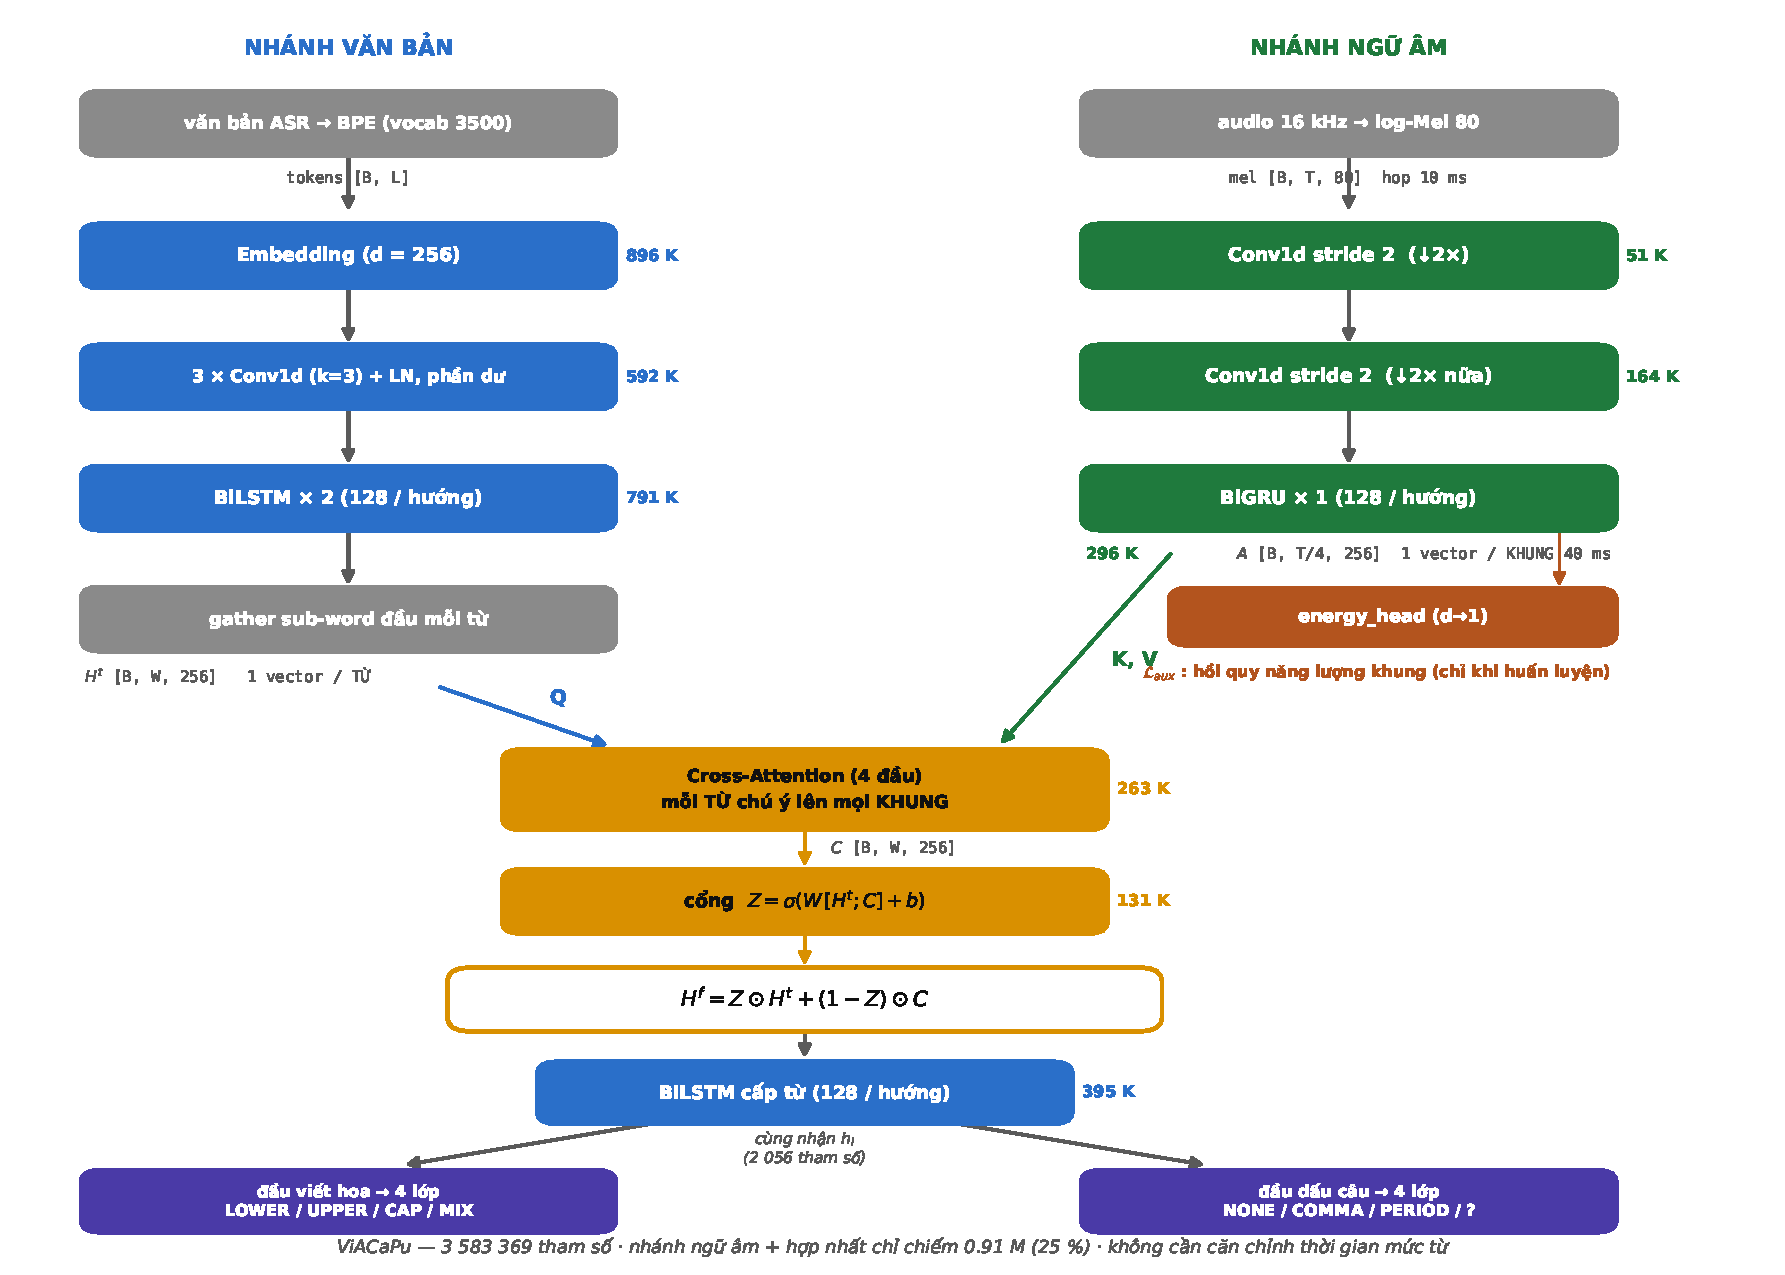
\includegraphics[width=0.92\textwidth]{figures/fig0_architecture.pdf}}
\caption{Kiến trúc ViACaPu, kèm số tham số của từng khối. Nhánh văn bản (trái) cho
ra một vector mỗi \emph{từ}; nhánh ngữ âm (phải) cho ra một vector mỗi \emph{khung}
40\,ms. Hai chuỗi có độ dài khác nhau gặp nhau ở cross-attention có cổng: trạng thái
từ đóng vai truy vấn, khung ngữ âm đóng vai khóa/giá trị, nên không cần dấu thời
gian mức từ. Đầu phụ \texttt{energy\_head} (cam) chỉ hoạt động khi huấn luyện và là
thành phần giúp nhánh ngữ âm đóng góp ổn định giữa các seed (Mục~\ref{sec:ablation}).}
\label{fig:arch}
\end{figure}

ViACaPu (Hình~\ref{fig:arch}) gồm bốn giai đoạn nối tiếp, tất cả dùng chung một số
chiều ẩn $d=256$:
\begin{enumerate}
\item[(1)] một \emph{nhánh văn bản} ánh xạ chuỗi sub-word thành một trạng thái cho
mỗi từ, $\mathbf{H}^{t}\in\mathbb{R}^{W\times d}$ (Mục~\ref{sec:text});
\item[(2)] một \emph{nhánh ngữ âm} ánh xạ phổ log-Mel thành một trạng thái cho mỗi
khung đã giảm mẫu, $\mathbf{A}\in\mathbb{R}^{T_a/4\times d}$ (Mục~\ref{sec:audio});
\item[(3)] một khối \emph{hợp nhất cross-attention có cổng} chiếu $\mathbf{A}$ về
lưới thời gian của $\mathbf{H}^{t}$ và trộn hai nguồn thành $\mathbf{H}^{f}
\in\mathbb{R}^{W\times d}$ (Mục~\ref{sec:fusion});
\item[(4)] một \emph{bộ giải mã cấp từ} với hai đầu ra song song sinh $(y^{c}_i,
y^{p}_i)$ (Mục~\ref{sec:decoder}).
\end{enumerate}
Điểm mấu chốt của thiết kế nằm ở giai đoạn (3): hai nhánh làm việc trên \emph{hai
lưới thời gian khác nhau} --- một chuỗi dài $W$ từ và một chuỗi dài $T_a/4$ khung
--- và cross-attention là thành phần duy nhất nối chúng lại. Vì phép nối này được
\emph{học} chứ không được cung cấp sẵn, mô hình thỏa mãn ràng buộc (R1). Nhánh ngữ
âm có thể được tắt hoàn toàn (\texttt{use\_acoustic}=\textsc{false}), khi đó
$\mathbf{H}^{f}\!=\!\mathbf{H}^{t}$ và phần còn lại không đổi; đây chính là biến
thể \emph{chỉ dùng văn bản} dùng trong các so sánh có kiểm soát ở
Mục~\ref{sec:results}.

\subsection{Nhánh văn bản}
\label{sec:text}
Bản ghi đã hạ chữ thường và bỏ dấu câu được token hóa bằng SentencePiece BPE (từ
điển 3\,500) thành $L$ sub-word. Chuỗi này đi qua một lớp nhúng $d$ chiều, rồi ba
khối tích chập phần dư một chiều ($k=3$, mỗi khối là $\mathbf{h}\!\leftarrow\!
\mathrm{LN}(\mathbf{h}+\mathrm{ReLU}(\mathrm{Conv1d}(\mathbf{h})))$) để nắm bắt các
mẫu hình thái cục bộ, và cuối cùng là một BiLSTM hai lớp (128 đơn vị mỗi hướng, nên
đầu ra ghép hai chiều vẫn có $d$ chiều) để mô hình hóa phụ thuộc tầm xa.

Việc chuyển từ lưới sub-word về lưới từ được thực hiện bằng phép \emph{gom theo vị
trí đầu từ}: với mỗi từ $i$, ta lấy trạng thái BiLSTM tại chỉ số sub-word đầu tiên
của từ đó,
\begin{equation}
\mathbf{H}^{t}_{i} = \mathbf{h}^{\mathrm{sub}}_{\pi(i)},\qquad i=1,\dots,W,
\end{equation}
với $\pi(i)$ là vị trí sub-word mở đầu từ thứ $i$. Do BiLSTM đã lan truyền thông
tin của các sub-word còn lại vào trạng thái này, phép gom không làm mất thông tin
nội bộ từ, đồng thời cho phép mọi giai đoạn phía sau làm việc trên một lưới cấp từ
duy nhất --- điều kiện để hai nhãn được gán chính xác một lần cho mỗi từ.

\subsection{Nhánh ngữ âm}
\label{sec:audio}
Nhánh này nhận phổ log-Mel 80 chiều (bước nhảy 10\,ms) và trả về đặc trưng khung
$\mathbf{A}$. Hai lớp tích chập một chiều stride-2 ($k=5$, kèm LayerNorm và ReLU)
lần lượt nâng số kênh $80\!\to\!d/2\!\to\!d$ và giảm độ phân giải thời gian
$4\times$, đưa bước khung hiệu dụng từ 10\,ms lên \textbf{40\,ms}. Chuỗi đã giảm
mẫu được mã hóa bởi một BiGRU một lớp (128 đơn vị mỗi hướng), cho
$\mathbf{A}\in\mathbb{R}^{T_a/4\times d}$.

Mức giảm mẫu $4\times$ là một lựa chọn có chủ đích. Các manh mối ngôn điệu liên
quan đến dấu câu --- khoảng lặng cuối mệnh đề, sự sụt giảm năng lượng, độ kéo dài
âm tiết trước ranh giới --- diễn ra ở thang \emph{hàng trăm mili-giây}, nên độ phân
giải 40\,ms vẫn dư sức biểu diễn chúng, trong khi chuỗi khóa/giá trị mà
cross-attention phải duyệt ngắn đi bốn lần. Với đoạn dài trung bình 5{,}3\,s, điều
này đưa $T_a$ từ $\approx530$ khung xuống $\approx133$, giảm chi phí attention
tương ứng.

\textbf{Đầu phụ dự đoán năng lượng.} Ngoài đường ra đặc trưng, bộ mã hóa ngữ âm có
thêm một phép chiếu tuyến tính $d\!\rightarrow\!1$ áp lên từng khung,
$\hat{e}_t = \mathbf{w}_e^{\top}\mathbf{A}_t + b_e$, sinh ra một chuỗi năng lượng
dự đoán $\hat{\mathbf{e}}\in\mathbb{R}^{T_a/4}$. Đầu này \emph{chỉ tồn tại trong
huấn luyện} và bị loại bỏ khi suy luận, nên không phát sinh chi phí triển khai.
Động cơ của nó là một vấn đề tối ưu chứ không phải vấn đề biểu diễn: nếu bộ mã hóa
ngữ âm chỉ nhận gradient gián tiếp thông qua cross-attention và mất mát CaPu, tín
hiệu học đi tới nó rất yếu ở giai đoạn đầu huấn luyện --- lúc mà cổng hợp nhất chưa
có lý do gì để mở về phía một biểu diễn ngữ âm còn ngẫu nhiên. Việc hồi quy trực
tiếp năng lượng khung buộc $\mathbf{A}$ mã hóa đường bao năng lượng (và do đó các
khoảng lặng) \emph{ngay từ những epoch đầu}, độc lập với trạng thái của cổng. Ảnh
hưởng định lượng của cơ chế này được phân tích ở Mục~\ref{sec:ablation}; ở đây chỉ
cần ghi nhận rằng đầu phụ là một dạng \emph{giám sát trung gian} nhằm ổn định quá
trình học của nhánh ngữ âm.

\subsection{Hợp nhất cross-attention có cổng}
\label{sec:fusion}
Giai đoạn này giải quyết trực tiếp ràng buộc (R1): làm sao đưa thông tin từ một
chuỗi $T_a/4$ khung về một chuỗi $W$ từ khi không biết từ nào ứng với khung nào.
Chúng tôi để \emph{mỗi trạng thái từ tự truy vấn} toàn bộ chuỗi khung:
\begin{align}
\mathbf{C} &= \mathrm{CrossAttn}(\mathbf{Q}{=}\mathbf{H}^{t},\;
              \mathbf{K}{=}\mathbf{V}{=}\mathbf{A}), \label{eq:xattn}\\
\mathbf{Z} &= \sigma\!\left(\mathbf{W}\,[\mathbf{H}^{t};\mathbf{C}] + \mathbf{b}\right), \label{eq:gate}\\
\mathbf{H}^{f} &= \mathbf{Z}\odot\mathbf{H}^{t} + (\mathbf{1}-\mathbf{Z})\odot\mathbf{C}. \label{eq:fuse}
\end{align}
Ở đây $\mathrm{CrossAttn}$ là multi-head attention chuẩn với 4 đầu; các khung nằm
ngoài độ dài thật của đoạn bị che bằng mặt nạ khóa. $[\,\cdot\,;\,\cdot\,]$ là phép
nối theo chiều đặc trưng, $\mathbf{W}\!\in\!\mathbb{R}^{d\times 2d}$ và
$\mathbf{b}\!\in\!\mathbb{R}^{d}$ là tham số của lớp cổng, $\sigma$ là sigmoid theo
từng phần tử và $\odot$ là tích Hadamard.

Hai phương trình đảm nhận hai vai trò tách bạch.
\eqref{eq:xattn} thực hiện \emph{căn chỉnh mềm}: trọng số attention
$\alpha_{it}\propto\exp(\mathbf{q}_i^{\top}\mathbf{k}_t/\sqrt{d_h})$ chính là một
phân bố học được trên các khung cho mỗi từ, thay thế cho dấu thời gian cứng mà ta
không có. Nhờ vậy mô hình không cần biết biên từ; nó chỉ cần học rằng trạng thái
của một từ ở cuối mệnh đề nên chú ý tới vùng khung theo sau nó, nơi chứa khoảng
lặng.
\eqref{eq:gate}--\eqref{eq:fuse} thực hiện \emph{điều tiết theo ngữ cảnh}: cổng
$\mathbf{Z}\!\in\![0,1]^{W\times d}$ quyết định, riêng cho từng từ và từng chiều
đặc trưng, nên tin vào bằng chứng văn bản hay bằng chứng ngữ âm. Khi
$\mathbf{Z}\!\to\!\mathbf{1}$ thì $\mathbf{H}^{f}\!\to\!\mathbf{H}^{t}$ và mô hình
suy biến về chế độ chỉ-văn-bản; khi $\mathbf{Z}\!\to\!\mathbf{0}$ thì biểu diễn
hợp nhất dựa hẳn vào ngữ cảnh ngữ âm $\mathbf{C}$. Tính chất này cần thiết vì hai
nguồn bằng chứng không đồng đều về độ tin cậy: với các từ mà cú pháp đã đủ xác định
dấu câu, ngữ âm là dư thừa; với các ranh giới mệnh đề mà văn bản mơ hồ --- điển
hình là dấu phẩy --- ngữ âm mới là tín hiệu quyết định. Một phép cộng hoặc nối cố
định sẽ áp cùng một tỉ lệ trộn cho mọi từ, trong khi cổng cho phép tỉ lệ đó thay
đổi theo từng vị trí. Giá trị cổng thực tế sau huấn luyện được phân tích ở
Mục~\ref{sec:ablation}.

\subsection{Bộ giải mã cấp từ và hai đầu ra}
\label{sec:decoder}
Chuỗi hợp nhất $\mathbf{H}^{f}$ đi qua một BiLSTM cấp từ một lớp (128 đơn vị mỗi
hướng) và dropout ($p=0{,}3$), cho trạng thái cuối $\mathbf{h}_i$ tại mỗi từ. Hai
phép chiếu tuyến tính độc lập $d\!\rightarrow\!4$ đọc \emph{cùng} một $\mathbf{h}_i$
để sinh logit cho hai tác vụ:
\begin{equation}
\hat{y}^{c}_i = \mathrm{softmax}(\mathbf{W}_c\mathbf{h}_i + \mathbf{b}_c),\qquad
\hat{y}^{p}_i = \mathrm{softmax}(\mathbf{W}_p\mathbf{h}_i + \mathbf{b}_p).
\end{equation}
Thiết kế này khác với~\cite{you2024lightweight}, vốn ghép trạng thái của \emph{từ
liền kề} cho mỗi đầu ra (đầu viết hoa nhìn cặp (trước, hiện tại), đầu dấu câu nhìn
cặp (hiện tại, sau)) nhằm đưa ngữ cảnh một phía vào từng tác vụ. Trong cấu hình của
chúng tôi, BiLSTM cấp từ đã tích hợp ngữ cảnh \emph{hai phía} vào $\mathbf{h}_i$,
nên phép ghép đó trở nên dư thừa; bỏ nó đi giữ kích thước đầu vào của hai đầu ở
mức $d$ thay vì $2d$, khiến toàn bộ phần đầu ra chỉ tốn 2\,056 tham số. Hai tác vụ
dùng chung toàn bộ thân mô hình và chỉ tách ở lớp cuối, phản ánh giả định rằng
viết hoa và dấu câu chia sẻ phần lớn bằng chứng cú pháp -- ngôn điệu.

Bốn lớp của mỗi tác vụ được lấy bằng cách gộp các ký hiệu hiếm về lớp gần nhất về
chức năng: ``!''$\rightarrow$PERIOD và ``;'',``:''$\rightarrow$COMMA. Cách gộp này
giữ số lớp nhỏ (phù hợp ngân sách tham số) mà không mất thông tin ngắt câu chính.

\subsection{Hàm mục tiêu}
\label{sec:objective}
Mô hình được huấn luyện đầu-cuối từ đầu (không dùng trọng số tiền huấn luyện) bằng
một mục tiêu đa nhiệm gồm ba số hạng:
\begin{equation}
\label{eq:loss}
\mathcal{L} = \underbrace{\mathcal{L}_{\mathrm{CE}}^{\mathrm{case}}}_{\text{viết hoa}}
            + \underbrace{0{,}7\,\mathcal{L}_{\mathrm{CE}}^{\mathrm{punct}}(\mathbf{w})}_{\text{dấu câu}}
            + \underbrace{\lambda_{\mathrm{aux}}\,\mathcal{L}_{\mathrm{MSE}}^{\mathrm{energy}}}_{\text{giám sát trung gian}}.
\end{equation}

\textbf{Hai số hạng tác vụ chính} là cross-entropy trên các vị trí từ. Cả hai chỉ
được tính trên \emph{những từ được chấm điểm}: các vị trí đệm, các sub-word không
phải đầu từ, cùng từ đầu và từ cuối của mỗi đoạn đều bị che. Hai từ biên bị loại
vì nhãn của chúng được xác định bởi ngữ cảnh nằm ngoài đoạn (từ đầu đoạn gần như
luôn viết hoa do vị trí, còn dấu câu sau từ cuối phụ thuộc câu kế tiếp), nên việc
chấm chúng sẽ thổi phồng điểm số một cách giả tạo. \emph{Cùng một mặt nạ này được
dùng lại khi đánh giá}, nên các con số ở Mục~\ref{sec:results} đo đúng những vị trí
mà mô hình thực sự được yêu cầu học.
Vector $\mathbf{w}=[1{,}0;\,1{,}6;\,1{,}05;\,1{,}4]$ là trọng số lớp cho
[NONE, COMMA, PERIOD, QUES], bù lại sự khan hiếm của COMMA và QUESTION trong phân
bố nhãn (Bảng~\ref{tab:data}); hệ số $0{,}7$ cân bằng đóng góp của hai tác vụ. Cả
hai giá trị đều được kế thừa từ~\cite{you2024lightweight} chứ không tinh chỉnh lại
(Mục~\ref{sec:hyper}).

\textbf{Số hạng giám sát trung gian} là sai số bình phương trung bình giữa chuỗi
năng lượng dự đoán $\hat{\mathbf{e}}$ (Mục~\ref{sec:audio}) và một mục tiêu năng
lượng tính trực tiếp từ đầu vào, không cần chú thích thêm:
\begin{equation}
e_t = \frac{1}{4}\sum_{j=4t}^{4t+3}\ \frac{1}{80}\sum_{m=1}^{80} \mathbf{X}^{a}_{j,m},
\qquad
\mathcal{L}_{\mathrm{MSE}}^{\mathrm{energy}}
  = \frac{1}{|\mathcal{T}|}\sum_{t\in\mathcal{T}} (\hat{e}_t - e_t)^2 ,
\end{equation}
tức lấy trung bình log-Mel theo chiều tần số để có năng lượng mỗi khung 10\,ms,
rồi gộp trung bình $4\times$ cho khớp bước giảm mẫu của bộ mã hóa; $\mathcal{T}$ là
tập khung hợp lệ của đoạn (bỏ phần đệm). Chúng tôi đặt
$\lambda_{\mathrm{aux}}=0{,}5$. Vì mục tiêu này được suy ra từ chính phổ đầu vào,
nó là một dạng \emph{tự giám sát} và không làm tăng yêu cầu dữ liệu. Đặt
$\lambda_{\mathrm{aux}}=0$ khôi phục đúng biến thể ``ngữ âm, không aux'' dùng trong
Bảng~\ref{tab:main}.

\subsection{Ngân sách tham số và chi phí của nhánh ngữ âm}
\label{sec:budget}
Bảng~\ref{tab:params} trình bày phân bố tham số theo mô-đun. Điểm đáng chú ý là
\emph{giá phải trả cho khả năng nhận biết ngữ âm}: bộ mã hóa ngữ âm (0{,}51M) cộng
khối hợp nhất (0{,}39M) chỉ chiếm \textbf{0{,}91 triệu tham số}, tức 25\,\% mô hình
và là phần chênh lệch giữa biến thể chỉ-văn-bản 2{,}68M và mô hình đầy đủ 3{,}58M.
Phần lớn ngân sách còn lại nằm ở nhánh văn bản và lớp nhúng; hai đầu ra gần như
không đáng kể (0{,}1\,\%). Vì so sánh chính ở Mục~\ref{sec:results} là giữa hai
biến thể chỉ khác nhau đúng 0{,}91M tham số này, mọi khác biệt hiệu năng giữa
chúng quy về đúng một yếu tố: sự có mặt của bằng chứng ngữ âm.

\begin{table}[htbp]
\caption{Phân bố tham số của ViACaPu ($d=256$).}
\label{tab:params}
\centering
\begin{tabular}{lrr}
\toprule
Mô-đun & Tham số & Tỉ lệ \\
\midrule
Nhúng ($3500\times256$)          & 896{,}000  & 25.0\,\% \\
BiLSTM văn bản (2 lớp)           & 790{,}528  & 22.1\,\% \\
Conv văn bản $\times3$ + LayerNorm & 592{,}128 & 16.5\,\% \\
Bộ mã hóa ngữ âm                 & 512{,}897  & 14.3\,\% \\
BiLSTM cấp từ                    & 395{,}264  & 11.0\,\% \\
Hợp nhất (cross-attention + cổng) & 394{,}496 & 11.0\,\% \\
Các đầu ra                       & 2{,}056    & \phantom{0}0.1\,\% \\
\midrule
\textbf{Tổng}                    & \textbf{3{,}583{,}369} & 100\,\% \\
\bottomrule
\end{tabular}
\end{table}

\section{Thiết Lập Thực Nghiệm}

\textbf{Nguồn dữ liệu.} Chúng tôi dùng bộ tiếng nói tiếng Việt công khai
\emph{Dolly-1000h}\footnote{\texttt{dolly-vn/dolly-audio-1000h-vietnamese} trên
HuggingFace.}, gồm các cặp (âm thanh, bản ghi có dấu câu) trải nhiều lĩnh vực.
\textbf{Cần nêu rõ một điểm quan trọng về bản chất dữ liệu:} theo thẻ metadata
chính thức của bộ dữ liệu (\texttt{tags: vietnamese, synthetic, audio, tts}),
âm thanh của Dolly-1000h là \emph{giọng nói tổng hợp bằng TTS}, không phải bản
ghi âm người nói thật, dù mô tả công khai của bộ dữ liệu nêu ``152 giọng đa
vùng miền'' theo cách dễ khiến người đọc hiểu nhầm là thu âm trực tiếp. Chúng
tôi không tìm thấy tài liệu công khai nào mô tả quy trình tổng hợp (hệ TTS nào,
có nhiều giọng huấn luyện hay clone giọng, hay tiền xử lý gì trước khi tổng
hợp). Vì các khoảng lặng và biến thiên năng lượng mà nhánh ngữ âm khai thác
(Mục~\ref{sec:audio}) có thể phản ánh quy luật chèn khoảng nghỉ của bộ tổng hợp
tiếng nói --- vốn thường mô hình hóa dấu câu một cách hệ thống hơn giọng nói tự
nhiên --- thay vì hành vi ngôn điệu tự nhiên của người nói, đây là một giới hạn
quan trọng của nghiên cứu (thảo luận thêm ở phần Hạn chế): mức cải thiện quan
sát được \emph{có thể không khái quát sang tiếng nói thu âm thật}. Sau khi lọc
các đoạn quá ngắn/quá dài, tập dữ liệu còn \textbf{658{,}128 đoạn} ($\approx$973
giờ âm thanh, 15.3 triệu từ).

\textbf{Chia tập.} Dữ liệu được chia 98/2 thành huấn luyện/kiểm định bằng một
phép hoán vị ngẫu nhiên cố định (\texttt{NumPy RandomState(42)}) trên toàn bộ
658\,128 đoạn (Bảng~\ref{tab:data}); mọi seed khởi tạo mô hình dùng chung phép
chia này để các lần chạy có thể so sánh trên cùng một tập. Chúng tôi nêu rõ ba
giới hạn của cách chia này. Thứ nhất, phép chia là theo \emph{đoạn}, không theo
người nói hay theo nguồn văn bản: siêu dữ liệu công khai của Dolly-1000h không
cung cấp nhãn định danh giọng nói hay định danh văn bản gốc cho từng đoạn, nên
chúng tôi không thể kiểm tra hay loại trừ khả năng cùng một giọng tổng hợp hoặc
cùng một câu nguồn xuất hiện ở cả hai tập. Với dữ liệu TTS, rủi ro này cao hơn
dữ liệu thu âm tự nhiên. Thứ hai, tập 2\,\% này đóng vai trò \emph{vừa chọn
checkpoint tốt nhất vừa báo cáo kết quả cuối}, nên các con số trong
Bảng~\ref{tab:main}--\ref{tab:seed} có thể lạc quan hơn một tập test hoàn toàn
độc lập. Để định lượng mức độ này, chúng tôi tách ngẫu nhiên tập kiểm định
13\,162 đoạn thành hai nửa bằng nhau (\emph{val-dev} để chọn checkpoint,
\emph{test} chỉ để báo cáo) và chấm lại các checkpoint đã huấn luyện trên từng
nửa; chênh lệch F1 dấu câu giữa hai nửa là nhỏ (từ $-0{,}003$ đến $+0{,}004$
qua các checkpoint được kiểm tra), cho thấy mức rò rỉ không lớn \emph{trong
phạm vi phép chia ngẫu nhiên theo đoạn này} --- nhưng phép kiểm tra này không
loại trừ được rủi ro trùng giọng/trùng văn bản nguồn nêu ở trên, vì cả hai nửa
đều lấy từ cùng một tập 2\,\% ban đầu. Thứ ba, vì thiếu định danh nguồn, chúng
tôi chưa kiểm tra được trùng lặp gần đúng (near-duplicate) giữa hai tập. Một
tập test độc lập, được chia theo giọng nói hoặc nguồn văn bản và không tham
gia bất kỳ bước chọn mô hình nào, là hướng thực nghiệm cần thiết tiếp theo.

\textbf{Sinh nhãn.} Từ mỗi bản ghi gốc có dấu câu, chúng tôi tách theo từ và gán
hai nhãn cho mỗi từ. Nhãn viết hoa được suy ra từ dạng chữ của từ
(LOWER/UPPER/CAP/MIX); nhãn dấu câu là ký hiệu \emph{đứng sau} từ, trong đó
``\,!\,''$\rightarrow$PERIOD và ``\,;\,'',``\,:\,''$\rightarrow$COMMA để gộp về
bốn lớp. Văn bản (đã hạ chữ thường, bỏ dấu câu) được token hóa bằng SentencePiece
BPE (từ điển 3500); chỉ sub-word đầu của mỗi từ mang nhãn, các sub-word còn lại
được che. Cần nhấn mạnh rằng chuỗi từ đưa vào mô hình được lấy từ chính \emph{bản ghi
tham chiếu} chứ không phải từ đầu ra của một bộ nhận dạng, nên mọi kết quả trong bài
tương ứng với kịch bản $\mathrm{WER}=0$ và là chặn trên của chất lượng triển khai. Phân bố nhãn lệch mạnh (Bảng~\ref{tab:data}), đặc biệt QUESTION chỉ
chiếm 0.25\,\% số vị trí được chấm điểm, thúc đẩy việc dùng trọng số lớp trong \eqref{eq:loss}
(Mục~\ref{sec:objective}).

\textbf{Đặc trưng âm học.} Âm thanh được lấy mẫu lại về 16\,kHz và trích phổ
log-Mel 80 chiều (cửa sổ 25\,ms, bước nhảy 10\,ms; \texttt{n\_fft}=400,
\texttt{hop}=160), sau đó chuẩn hóa trung bình--phương sai theo từng đoạn. Chuỗi
khung được nhánh ngữ âm giảm mẫu $4\times$ (Mục~\ref{sec:audio}).

\begin{table}[htbp]
\caption{Thống kê bộ dữ liệu Dolly-1000h. Tần suất nhãn được tính trên
\emph{tập vị trí được chấm điểm} (14.03 triệu từ, đã loại hai từ biên của mỗi
đoạn theo Mục~\ref{sec:objective}), chứ không phải trên toàn bộ 15.35 triệu nhãn
--- vì đó mới là phân bố mà hàm mất mát và các chỉ số thực sự nhìn thấy. Nếu
tính trên toàn bộ, NONE là 91.6\,\% và QUES là 0.23\,\%.}
\label{tab:data}
\centering
\setlength{\tabcolsep}{8pt}
\begin{tabular}{lr}
\toprule
Thuộc tính & Giá trị \\
\midrule
Số đoạn (train / val)        & 644{,}966 / 13{,}162 \\
Tổng thời lượng âm thanh     & 973.4 giờ \\
Độ dài đoạn (TB / trung vị / max) & 5.32 / 4.70 / 16.0\,s \\
Tổng số từ có nhãn           & 15.35 triệu \\
\quad trong đó \emph{được chấm điểm}  & 14.03 triệu \\
\midrule
Tần suất PUNCT (\%) & \\
\quad NONE / COMMA / PERIOD / QUES & 90.80 / 4.10 / 4.86 / 0.25 \\
Tần suất CASE (\%) & \\
\quad LOWER / UPPER / CAP / MIX    & 91.70 / 0.12 / 8.17 / 0.01 \\
\bottomrule
\end{tabular}
\end{table}

\textbf{Huấn luyện.} Adam, tốc độ học $8\times10^{-4}$, weight decay
$5\times10^{-5}$, cosine annealing trong 12 epoch, kích thước batch 64. Một GPU
NVIDIA RTX~3060 (12\,GB) huấn luyện ViACaPu trong khoảng 1.5\,giờ. Checkpoint
được chọn là epoch cực đại hóa \emph{tổng} hai chỉ số (F1 viết hoa $+$ F1 dấu
câu) trên tập kiểm định; chúng tôi nêu rõ điều này vì bài báo cáo riêng từng chỉ
số, trong khi tiêu chí chọn là tiêu chí gộp. Mọi cấu hình trong bài dùng chung
tiêu chí này, nên các so sánh giữa chúng không bị lệch bởi lựa chọn đó.

\textbf{Độ đo.} Mọi điểm số đều được tính ở mức \emph{từ}: mỗi vị trí từ thật đóng
góp đúng một dự đoán viết hoa và một dự đoán dấu câu (bỏ padding và các sub-word
không phải đầu từ). Với một lớp $c$, gọi $TP_c$ là số từ được gán đúng vào lớp $c$,
$FP_c$ là số từ bị gán nhầm vào $c$, và $FN_c$ là số từ thực sự thuộc lớp $c$ nhưng
mô hình gán sang lớp khác. Precision, recall và trung bình điều hòa của chúng là
\begin{equation}
P_c = \frac{TP_c}{TP_c + FP_c},\quad
R_c = \frac{TP_c}{TP_c + FN_c},\quad
F1_c = \frac{2\,P_c R_c}{P_c + R_c}.
\end{equation}
Một cách trực quan, $P_c$ trả lời \emph{trong những trường hợp mô hình dự đoán là
$c$, bao nhiêu phần là đúng}, còn $R_c$ trả lời \emph{trong những trường hợp thực
sự là $c$, mô hình tìm ra được bao nhiêu}; $F1_c$ cân bằng cả hai và sẽ thấp ngay
khi một trong hai thấp. Điều này quan trọng ở đây vì hai loại lỗi có chi phí khác
nhau: bỏ sót một dấu phẩy khiến văn bản thiếu ngắt nghỉ, trong khi thêm một dấu
phẩy thừa lại chủ động làm người đọc hiểu sai.

Điểm dấu câu \emph{tổng thể} là trung bình \textbf{micro} chỉ trên ba lớp mang
thông tin $\mathcal{C}=\{$COMMA, PERIOD, QUESTION$\}$, tức là gộp các đếm số trước
rồi mới lấy tỉ lệ:
\begin{equation}
P = \frac{\sum_{c \in \mathcal{C}} TP_c}{\sum_{c \in \mathcal{C}} (TP_c + FP_c)},
\quad
R = \frac{\sum_{c \in \mathcal{C}} TP_c}{\sum_{c \in \mathcal{C}} (TP_c + FN_c)},
\end{equation}
và $F1$ được tạo từ hai đại lượng này như trên. Lớp NONE chiếm đa số được cố ý loại
trừ: nó chiếm 90.8\,\% tổng số từ (Bảng~\ref{tab:data}), nên nếu tính cả nó thì một
mô hình chỉ việc dự đoán NONE ở mọi vị trí cũng đạt trên 0.90 mà không khôi phục
được dấu câu nào. Điểm viết hoa được tính tương tự trên $\{$UPPER, CAP, MIX$\}$,
loại LOWER vì cùng lý do. Trung bình micro có trọng số theo tần suất lớp, nên con
số tổng thể phản ánh đúng những dấu câu mà người đọc thực sự gặp; $F1$ theo từng
lớp (Bảng~\ref{tab:perclass}) được báo cáo kèm chính vì các lớp hiếm sẽ bị che
khuất nếu chỉ nhìn con số tổng.

\textbf{Mô hình cơ sở.} (a)~Mô hình chỉ dùng văn bản của~\cite{you2024lightweight}
(7.26 triệu tham số theo bản cài đặt lại của chúng tôi), được huấn luyện lại trên
Dolly để so sánh cùng miền;
(b)~ViACaPu với nhánh ngữ âm bị tắt (2.68 triệu), một phép ablation chia sẻ y hệt
nhánh văn bản và các đầu ra.

\textbf{Lý giải các siêu tham số.}\label{sec:hyper}
(i)~\emph{Trọng số mất mát $0.7$}: chúng tôi kế thừa giá trị này từ mô hình
gốc~\cite{you2024lightweight} để giữ thiết lập đa nhiệm gần với công trình cơ sở;
giá trị này không được tinh chỉnh lại riêng trên Dolly. (ii)~\emph{Độ rộng
$d=256$}: đây là giá trị mặc định mà chúng tôi cố định ngay từ đầu và \emph{không}
phải kết quả của một phép tìm kiếm; chúng tôi nêu rõ điều này để tránh diễn giải
hồi tố. Bề rộng duy nhất được thử thêm là $d=384$; khi giữ nguyên mất mát phụ để
chỉ đổi một biến, bề rộng này cho F1 dấu câu $0{,}928$, tức ngang mức $0{,}927$
của $d=256$ với gần gấp đôi số tham số (Mục~\ref{sec:capacity}).
Các bề rộng nhỏ hơn ($d\in\{128,192\}$, tương ứng 1.14M và 2.20M tham số) chưa được
đánh giá; vì mục tiêu của bài là mô hình cho thiết bị biên, đây là hướng đáng theo
đuổi hơn là mở rộng mô hình.
(iii)~\emph{Trọng số lớp $[1.0,1.6,1.05,1.4]$}: COMMA và QUESTION là các lớp hiếm
nên được tăng trọng số so với NONE nhằm giảm ảnh hưởng của mất cân bằng nhãn; các
trọng số này được đặt thủ công, không diễn giải như nghịch đảo chính xác của tần
suất lớp, và \emph{chưa} được so sánh với biến thể không trọng số bằng ablation
riêng. (iv)~Các siêu tham số còn lại (số bộ lọc/kích thước kernel của khối tích
chập, số đơn vị và số lớp của các mạng hồi quy) được kế thừa
từ~\cite{you2024lightweight} và không được tìm kiếm lại.
Tốc độ học, weight decay và số epoch theo cấu hình chuẩn, không tinh chỉnh riêng.

Chúng tôi nêu rõ giới hạn của phần này: các giá trị siêu tham số ở trên chủ yếu
được \emph{kế thừa hoặc chọn theo một tập cấu hình giới hạn}, chứ chưa được tìm
kiếm có hệ thống trên Dolly. Cụ thể, hệ số mất mát $0.7$ và trọng số lớp chưa được
quét; bề rộng $d$ mới được đánh giá ở $\{256, 384\}$ chứ chưa phải một dải mịn
(ví dụ $128,192,256,320,384$), và các bề rộng \emph{nhỏ hơn} $256$ --- hướng
đáng quan tâm nhất với mục tiêu thiết bị biên --- chưa được thử. Do đó, chúng tôi \emph{không} tuyên bố bộ siêu tham
số hiện tại là tối ưu; việc tìm kiếm siêu tham số đầy đủ để xác nhận (hoặc cải
thiện) lựa chọn này là một hướng thực nghiệm tiếp theo. Các kết luận chính của bài
báo (Mục~\ref{sec:results}) dựa trên các \emph{so sánh có kiểm soát cùng một cấu
hình}, nên không phụ thuộc vào giả định rằng cấu hình đó đã tối ưu.

\section{Kết Quả}
\label{sec:results}

\subsection{So sánh tổng quan}

\begin{table}[htbp]
\caption{Kết quả trên Dolly (tiếng Việt), \emph{tất cả} đánh giá trên cùng một tập
kiểm định 13\,162 đoạn (chia theo seed 42). Mô hình cơ sở~\cite{you2024lightweight}
được huấn luyện lại trên Dolly bằng cùng bộ token hóa và cùng quy ước nhãn, nhưng
\emph{giữ nguyên công thức huấn luyện gốc của nó} --- khác ViACaPu ở hai điểm
(không dùng trọng số lớp; không loại hai từ biên khỏi mất mát và khỏi phép chấm)
--- nên dòng này là \emph{đối chiếu tham khảo}, không phải ablation đổi một biến;
xem phần thảo luận sau bảng. Ba dòng ViACaPu khác nhau \emph{đúng} ở nhánh ngữ âm
và mất mát phụ, nên các so sánh giữa chúng là có kiểm soát. Số tham số của mô hình
cơ sở là do chúng tôi đếm từ bản cài đặt lại, vì bài gốc chỉ công bố kích thước
ONNX. Ba dòng ViACaPu là trung bình\,$\pm$\,độ lệch chuẩn trên 3 seed. Phép so
sánh dung lượng nằm ở Bảng~\ref{tab:ablation}.}
\label{tab:main}
\centering
\setlength{\tabcolsep}{6pt}
\begin{tabular}{lrccc}
\toprule
Mô hình & Tham số & F1 hoa & F1 câu & COMMA \\
\midrule
Cơ sở~\cite{you2024lightweight}      & 7.26M & 0.936 & 0.569 & 0.634 \\
ViACaPu (chỉ văn bản)                & 2.68M & 0.937\,\tiny$\pm$.001 & 0.820\,\tiny$\pm$.002 & 0.660\,\tiny$\pm$.003 \\
ViACaPu (ngữ âm, không aux)          & 3.58M & 0.940\,\tiny$\pm$.003 & 0.854\,\tiny$\pm$.059 & 0.731\,\tiny$\pm$.124 \\
\textbf{ViACaPu (ngữ âm\,+\,aux)}    & \textbf{3.58M} & \textbf{0.944\,\tiny$\pm$.002} & \textbf{0.927\,\tiny$\pm$.004} & \textbf{0.888\,\tiny$\pm$.007} \\
\bottomrule
\end{tabular}
\end{table}

Bảng~\ref{tab:main} và Hình~\ref{fig:compare} tóm tắt kết quả chính. Đóng góp cốt
lõi của bài báo là một mô hình CaPu \emph{vừa nhẹ vừa chất lượng cao} cho thiết bị
biên; nhánh ngữ âm --- khi được dẫn dắt bằng mất mát phụ năng lượng --- là một
trong các phương pháp để đạt mục tiêu đó. Phép so sánh có kiểm soát chặt chẽ nhất
là giữa các biến thể ViACaPu (cùng nhánh văn bản, cùng đầu ra, cùng tập kiểm định
âm thanh). So với biến thể chỉ dùng văn bản, thêm nhánh ngữ âm với mất mát phụ nâng
F1 dấu câu \textbf{+0.107} và F1 dấu phẩy \textbf{+0.228} (chênh lệch ghép cặp theo
seed, nhất quán qua cả ba seed) chỉ với 0.91 triệu tham số bổ sung (Mục~\ref{sec:budget}). Đáng chú ý, khi
\emph{không} có mất mát phụ, cùng kiến trúc ngữ âm chỉ engage ở \emph{một trong
ba seed} (0.922 so với 0.819 và 0.820, tức hai seed rơi đúng về mức chỉ-văn-bản);
con số trung bình 0.854 trong bảng vì vậy không ứng với lần chạy nào và được ghi
kèm chỉ để đối chiếu --- hiện tượng này được phân tích ở Mục~\ref{sec:ablation}.

So với mô hình cơ sở~\cite{you2024lightweight} (7.26 triệu tham số theo bản cài đặt
lại của chúng tôi, huấn luyện lại trên Dolly và chấm trên \emph{cùng} tập kiểm
định), ViACaPu\,+\,aux tuy \emph{nhỏ hơn} (3.58 triệu) nhưng cao hơn nhiều ở dấu
câu: F1 câu $0.569 \to 0.927$ và COMMA $0.634 \to 0.888$. Hai mô hình gần nhau ở
viết hoa (F1 hoa $0.936$ so với $0.944$) --- một tác vụ chủ yếu dựa vào manh mối
từ vựng --- nhưng cách biệt lớn ở dấu câu. Tuy vậy, khoảng cách này \emph{không}
quy hết được cho nhánh ngữ âm: hai mô hình còn khác nhau ở công thức mất mát và
quy ước chấm điểm, như phân tích ngay dưới đây.

\textbf{Vì sao khoảng cách $0{,}569 \to 0{,}820$ chưa được quy trách nhiệm.}
Chúng tôi trình bày rõ giới hạn của phép đối chiếu này, vì khoảng cách trên
\emph{lớn hơn} cả đóng góp của nhánh ngữ âm ($+0{,}107$) và do đó cần được
diễn giải thận trọng. Hai yếu tố đã được loại trừ: bộ mã hóa SentencePiece
(\texttt{bpe.model}, từ điển 3\,500) và quy ước gộp nhãn dấu câu là
\emph{giống hệt} giữa hai mô hình, nên chênh lệch không đến từ token hóa; và
vì mô hình cơ sở \emph{lớn hơn gấp đôi} ViACaPu mà vẫn kém hơn, chênh lệch
cũng không quy được cho dung lượng.

Phần còn lại lẫn \emph{ít nhất bốn} biến mà thí nghiệm hiện tại không tách
được. Hai biến thuộc về \emph{công thức huấn luyện}, và chúng tôi cho rằng đây
là các ứng viên có khả năng nhất: \emph{(i)} mô hình cơ sở dùng cross-entropy
\emph{không trọng số lớp}, trong khi ViACaPu tăng trọng số COMMA và QUESTION
(\eqref{eq:loss}) --- với phân bố lệch 90.8\,\% NONE, đây chính là can thiệp
tác động trực tiếp lên xu hướng mô hình dám dự đoán lớp hiếm, và F1 COMMA
$0{,}634$ của mô hình cơ sở đi kèm recall thấp đúng như triệu chứng của việc
không bù mất cân bằng; \emph{(ii)} mô hình cơ sở chấm điểm trên \emph{toàn bộ}
vị trí, trong khi ViACaPu loại hai từ biên khỏi cả mất mát lẫn phép chấm
(Mục~\ref{sec:objective}), nên hai mô hình không được đánh giá trên cùng một
tập vị trí. Hai biến còn lại thuộc về \emph{kiến trúc}: \emph{(iii)}
\texttt{dropout} nhẹ hơn ($0{,}3$ so với $0{,}5$); và \emph{(iv)} mô hình cơ
sở \emph{cố ý tránh self-attention}, theo ghi chú của chính tác giả trong mã
nguồn công khai (\textit{``use attention will predict `how are you' as `How?
are? you?', seems not suitable for this model''}).

Vì \emph{(i)} và \emph{(ii)} là khác biệt về cách huấn luyện và cách chấm chứ
không phải về năng lực kiến trúc, chúng tôi \emph{không} tuyên bố rằng khoảng
cách $0{,}569 \to 0{,}820$ đo được ưu thế kiến trúc của nhánh văn bản ViACaPu.
Việc huấn luyện lại mô hình cơ sở dưới đúng công thức mất mát và đúng quy ước
chấm điểm của ViACaPu là phép kiểm chứng cần thiết mà chúng tôi chưa thực
hiện. Cần nhấn mạnh rằng giới hạn này \emph{không} ảnh hưởng tới các kết luận
chính của bài: toàn bộ lưới tách biến (Mục~\ref{sec:ablation}) và ablation
dung lượng (Mục~\ref{sec:capacity}) chỉ so sánh các biến thể ViACaPu dùng
chung y hệt công thức mất mát, mặt nạ chấm điểm và cách chia tập.

\begin{figure}[htbp]
\centering
\centerline{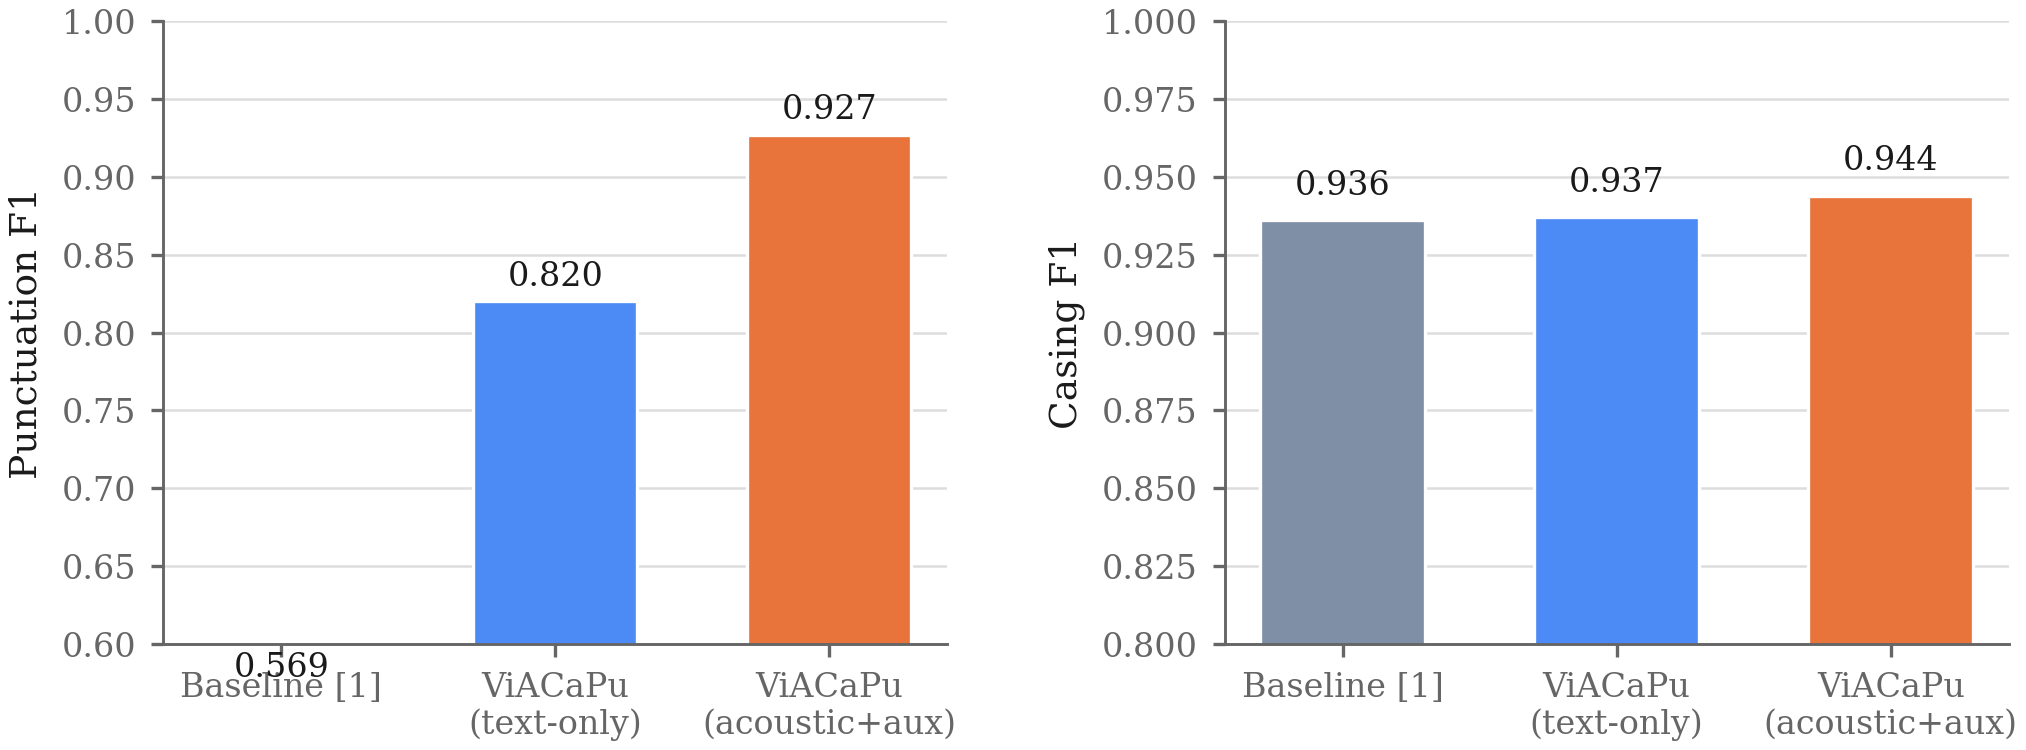
\includegraphics[width=0.72\textwidth]{figures/fig1_compare_all_models.png}}
\caption{F1 dấu câu và viết hoa trên Dolly, tất cả trên cùng một tập kiểm định.
Cả ba mô hình gần nhau ở viết hoa nhưng cách biệt lớn ở dấu câu; ViACaPu\,+\,aux
(3.58M) vượt mô hình cơ sở 7.26M dù nhỏ hơn.}
\label{fig:compare}
\end{figure}

\subsection{Phân tích theo lớp}

\begin{table}[htbp]
\caption{Kết quả dấu câu theo lớp của ViACaPu (ngữ âm\,+\,aux) trên Dolly, một seed
đại diện.}
\label{tab:perclass}
\centering
\begin{tabular}{lccc}
\toprule
Lớp & Precision & Recall & F1 \\
\midrule
COMMA        & 0.877 & 0.910 & 0.893 \\
PERIOD       & 0.984 & 0.955 & 0.969 \\
QUESTION     & 0.777 & 0.737 & 0.756 \\
\midrule
\textbf{Tổng} & 0.930 & 0.930 & \textbf{0.930} \\
\bottomrule
\end{tabular}
\end{table}

Hình~\ref{fig:perclass} và Bảng~\ref{tab:perclass} định vị phần cải thiện. Các ma
trận nhầm lẫn trong Hình~\ref{fig:cmpunct} minh họa rõ hơn: mô hình chỉ dùng văn
bản bỏ sót phần lớn dấu phẩy (dự đoán thành NONE), trong khi mô hình ngữ âm\,+\,aux
bỏ sót ít hơn nhiều --- nâng recall dấu phẩy từ 0.657 lên 0.910. Đây chính là hành
vi mà giả thuyết về khoảng lặng dự đoán. Ngược lại, viết hoa gần như không bị ảnh
hưởng (Hình~\ref{fig:cmcase}), khẳng định rằng viết hoa là hiện tượng chủ yếu mang
tính từ vựng.

\begin{figure}[htbp]
\centering
\centerline{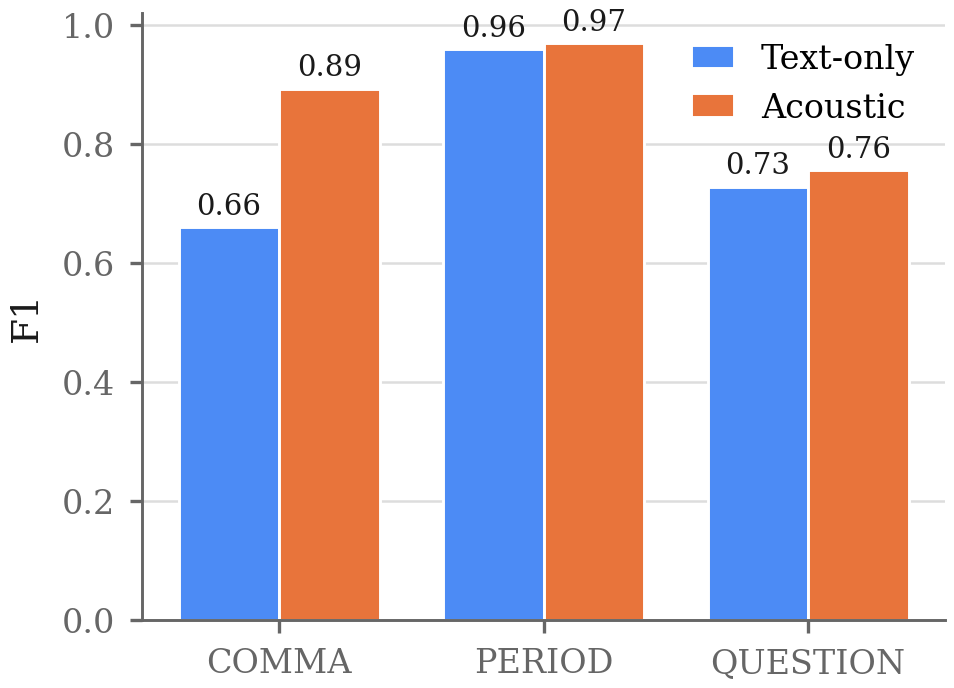
\includegraphics[width=0.72\textwidth]{figures/fig2_punct_f1_perclass.png}}
\caption{F1 dấu câu theo lớp. Lợi ích của ngữ âm tập trung ở COMMA.}
\label{fig:perclass}
\end{figure}

\begin{figure}[htbp]
\centering
\centerline{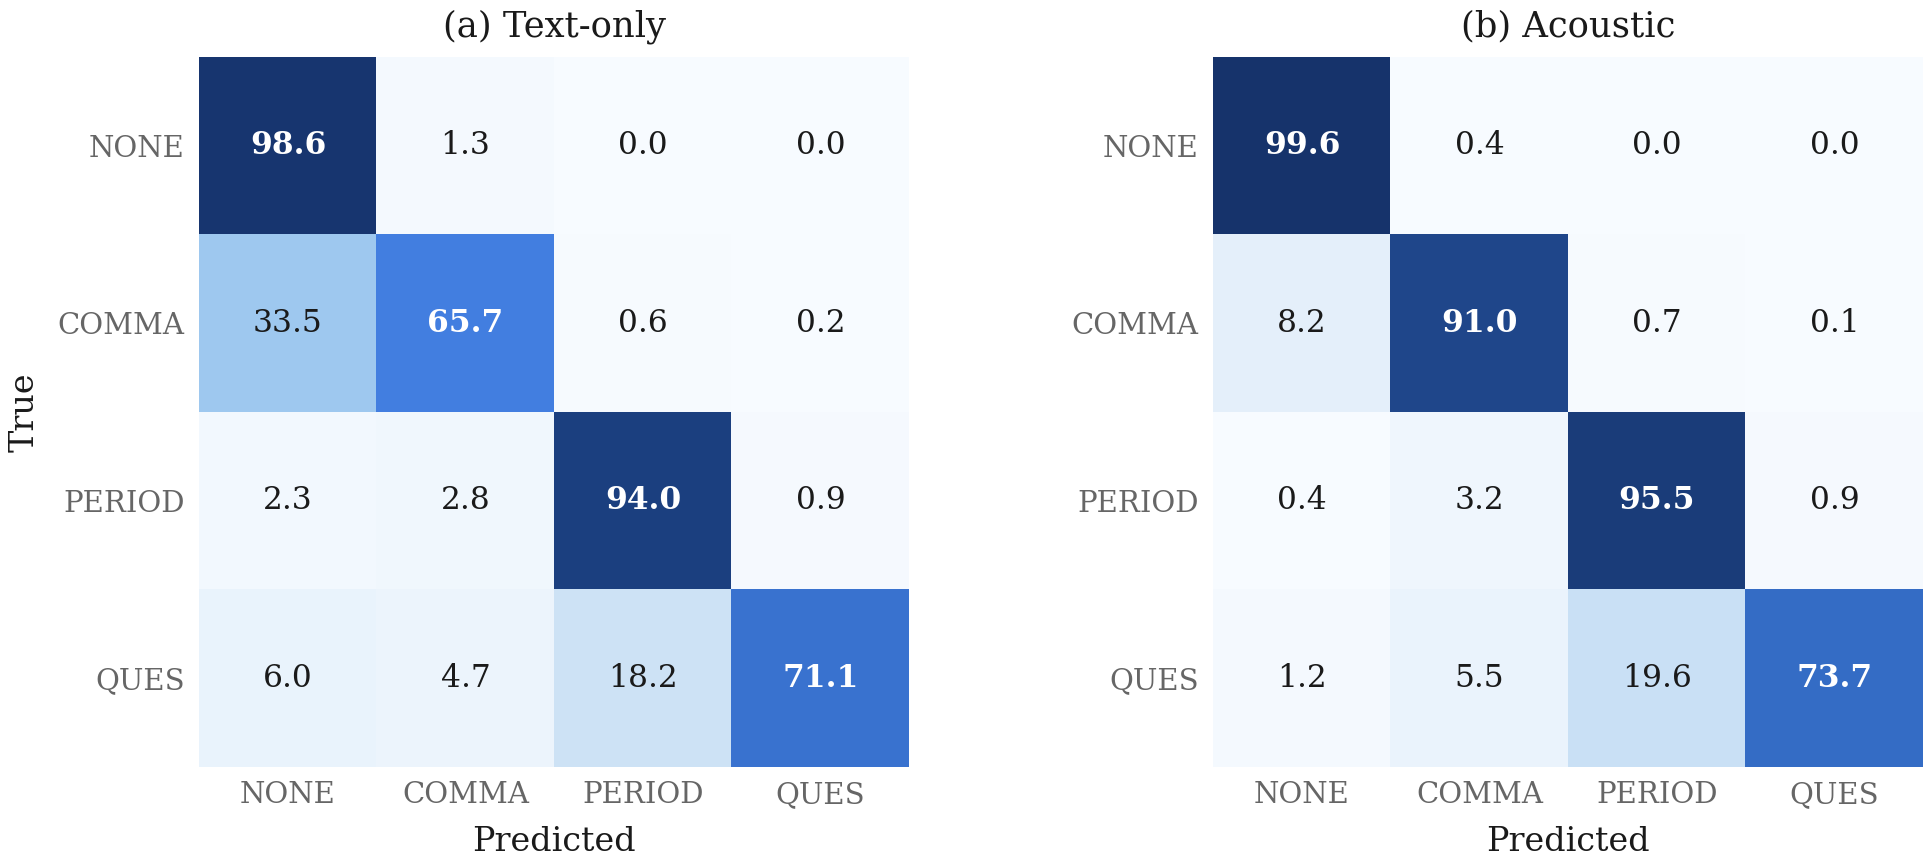
\includegraphics[width=0.72\textwidth]{figures/fig3_confusion_punct_acoustic.png}}
\caption{Ma trận nhầm lẫn dấu câu (chuẩn hóa theo hàng). (a) Chỉ dùng văn bản so
với (b) ngữ âm; mỗi ô báo cáo phần trăm theo hàng.}
\label{fig:cmpunct}
\end{figure}

\begin{figure}[htbp]
\centering
\centerline{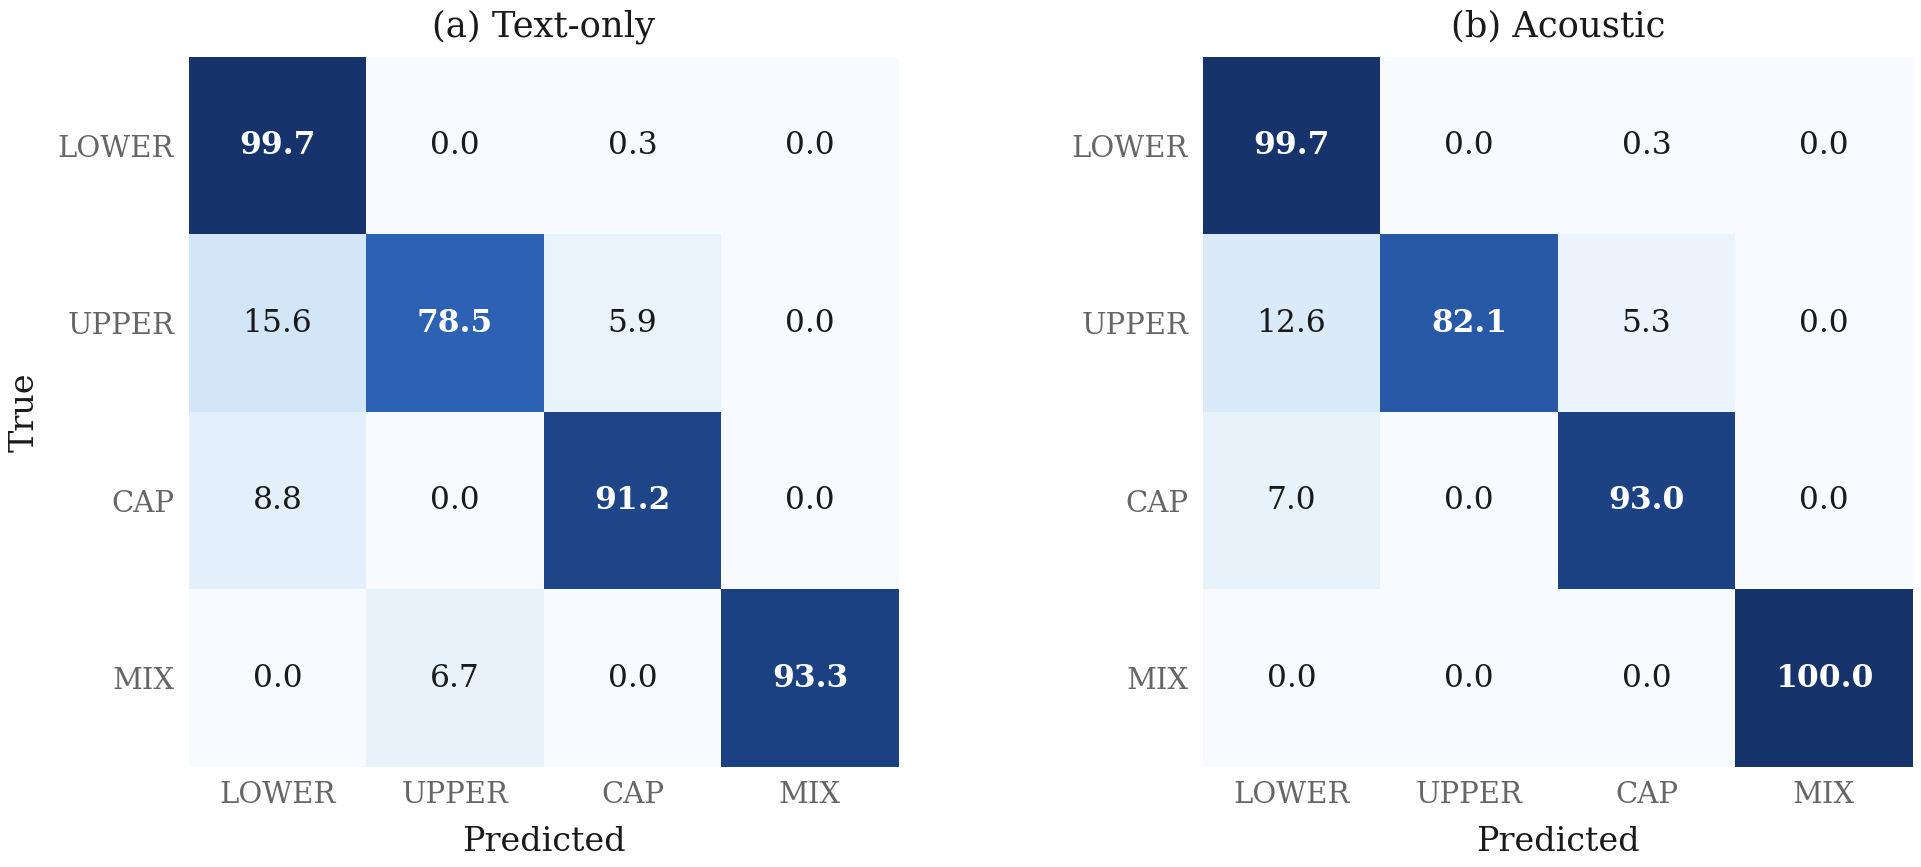
\includegraphics[width=0.72\textwidth]{figures/fig4_confusion_case_acoustic.png}}
\caption{Ma trận nhầm lẫn viết hoa. Hai biến thể gần như trùng khớp.}
\label{fig:cmcase}
\end{figure}

\subsection{Độ ổn định theo seed và vai trò của mất mát phụ}
\label{sec:ablation}

Trong các thí nghiệm ban đầu, chúng tôi quan sát thấy nhánh ngữ âm cải thiện mạnh ở
một số lần chạy nhưng gần như không đóng góp gì ở các lần khác. Để tìm nguyên nhân,
chúng tôi chạy một lưới $2\times2$ tách riêng hai can thiệp từng được áp dụng cùng
lúc: \emph{(i)} khởi tạo bias của cổng hợp nhất ở giá trị âm ($-2{,}0$) để ép nhiều
ngữ cảnh ngữ âm chảy vào từ sớm, và \emph{(ii)} mất mát phụ dự đoán năng lượng khung
($\lambda_{\mathrm{aux}}=0{,}5$). Mỗi ô của lưới được huấn luyện lại với ba seed
khởi tạo, giữ nguyên dữ liệu, cách chia tập và công thức huấn luyện; tập kiểm định
cố định theo seed 42 nên mọi lần chạy được chấm trên cùng một tập.

\begin{table}[htbp]
\caption{Lưới tách biến qua 3 seed (F1 dấu câu, trung bình\,$\pm$\,độ lệch chuẩn mẫu;
cột ``seeds'' liệt kê giá trị của seed 42/43/44). Khởi tạo cổng \emph{một mình}
không mang lại lợi ích nào; mất mát phụ \emph{một mình} đã đủ để thu hẹp biến thiên
giữa các seed. Với dòng ``Ngữ âm'' ($\lambda_{\mathrm{aux}}{=}0$), cột trung bình
$\pm$ độ lệch chuẩn \emph{không} mô tả đúng dữ liệu: ba seed phân thành hai cụm
tách biệt ($0{,}922$ so với $\approx\!0{,}82$) chứ không phân tán quanh một giá
trị trung tâm --- nên cần đọc cột ``seeds'' thay vì cột trung bình.}
\label{tab:seed}
\centering
\setlength{\tabcolsep}{5pt}
\begin{tabular}{llccccc}
\toprule
Cấu hình & bias cổng & $\lambda_{\mathrm{aux}}$ & F1 câu & seeds & F1 hoa & COMMA \\
\midrule
Chỉ văn bản                & ---        & ---   & 0.820\,$\pm$\,0.002 & 0.820/0.819/0.822 & 0.937 & 0.660\,$\pm$\,0.003 \\
Ngữ âm                     & mặc định   & 0     & 0.854\,$\pm$\,0.059 & 0.922/0.819/0.820 & 0.940 & 0.731\,$\pm$\,0.124 \\
Ngữ âm + bias cổng         & $-2{,}0$   & 0     & 0.818\,$\pm$\,0.001 & 0.817/0.819/0.818 & 0.938 & 0.658\,$\pm$\,0.001 \\
Ngữ âm + aux               & mặc định   & 0.5   & 0.926\,$\pm$\,0.003 & 0.924/0.929/0.924 & 0.944 & 0.885\,$\pm$\,0.007 \\
\textbf{Ngữ âm + bias + aux} & $-2{,}0$ & 0.5   & \textbf{0.927\,$\pm$\,0.004} & 0.928/0.930/0.923 & \textbf{0.944} & \textbf{0.888\,$\pm$\,0.007} \\
\bottomrule
\end{tabular}
\end{table}

\begin{figure}[htbp]
\centering
\centerline{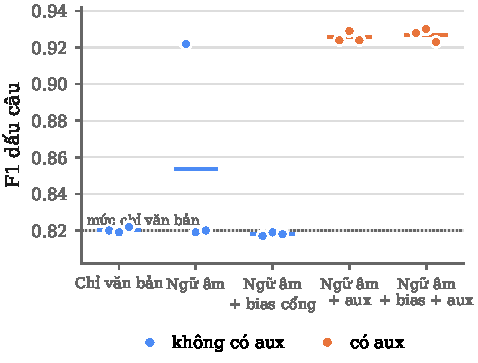
\includegraphics[width=0.62\textwidth]{figures/fig7_disentangle.pdf}}
\caption{Lưới tách biến: mỗi điểm là một seed, vạch ngang là trung bình ba seed.
Hai cấu hình \emph{không} có mất mát phụ (xanh) hoặc phân tán rộng theo seed, hoặc
nằm đúng mức chỉ-văn-bản; bật mất mát phụ (cam) vừa nâng trung bình vừa thu hẹp
biến thiên. Khởi tạo bias cổng một mình không tách khỏi đường chấm chỉ-văn-bản.}
\label{fig:disentangle}
\end{figure}

Bảng~\ref{tab:seed} và Hình~\ref{fig:disentangle} cho phép đọc ra ba điều, mỗi điều
ứng với một phép so sánh chỉ đổi một biến.

\textbf{Thứ nhất, nhánh ngữ âm không được giám sát cho hành vi lưỡng cực, chứ
không phải nhiễu quanh một trung bình.} Khi chỉ bật nhánh ngữ âm mà không có can
thiệp nào, ba seed không phân tán đều mà rơi vào \emph{hai chế độ tách biệt}:
seed 42 đạt $0{,}922$ (nhánh ngữ âm ``engage''), còn hai seed còn lại cho
$0{,}819$ và $0{,}820$ --- trùng khít mức chỉ-văn-bản, tức nhánh ngữ âm thực tế
không đóng góp gì. Không seed nào nằm ở khoảng giữa. Vì vậy con số
$0{,}854\pm0{,}059$ ở Bảng~\ref{tab:seed} nên được hiểu là \emph{tỉ lệ thành
công} (một trong ba lần chạy) chứ không phải một mức chất lượng kỳ vọng: không
có cấu hình nào thực sự đạt $0{,}854$. Nếu chỉ nhìn một lần chạy thuận lợi, ta
sẽ kết luận sai rằng nhánh ngữ âm luôn giúp $+0{,}10$; nếu chỉ nhìn một lần chạy
không thuận lợi, ta sẽ kết luận sai rằng ngữ âm vô dụng.

\textbf{Thứ hai, việc mở cổng không phải là nguyên nhân.} Trực giác ban đầu của
chúng tôi là cổng hợp nhất đóng lại với luồng ngữ âm (``gate collapse''), nên chúng
tôi khởi tạo bias cổng ở $-2{,}0$ để ép cổng mở. Can thiệp này \emph{không cải thiện
gì}: $0{,}818\pm0{,}001$, trùng khít mức chỉ-văn-bản ở cả ba seed, và F1 dấu phẩy
($0{,}658$) cũng ngang mức đó. Phép đo giá trị cổng đồng thuận với kết quả này: cả
seed ``thắng'' lẫn hai seed ``thua'' đều có $\mathbf{Z}\!\approx\!0{,}57$--$0{,}65$
(trung bình trên mọi từ và mọi chiều đặc trưng), tức trung bình $35$--$43\,\%$
biểu diễn hợp nhất đến từ ngữ cảnh ngữ âm ở \emph{mọi} seed --- cổng không hề
đóng lại. Chúng tôi lưu ý rằng đây là một thống kê tổng hợp: nó loại trừ kịch
bản cổng đóng đồng loạt, nhưng không loại trừ được khả năng cổng mở không đồng
đều giữa các chiều đặc trưng; phân tích phân bố của $\mathbf{Z}$ theo chiều chưa
được thực hiện. Dù vậy, kết luận cần thiết ở đây đã đủ vững: ngữ âm vẫn được nạp
vào, nên vấn đề nằm ở \emph{nội dung} mà bộ mã hóa ngữ âm học được, không phải ở
lưu lượng.

\textbf{Thứ ba, mất mát phụ là thành phần tạo ra hiệu quả.} Bật riêng mất mát phụ,
không kèm can thiệp cổng, đã nâng F1 dấu câu lên $0{,}926\pm0{,}003$ và COMMA lên
$0{,}885\pm0{,}007$; hai seed vốn ``thua'' được kéo lên ngang seed thuận lợi
($0{,}929$ và $0{,}924$). Chênh lệch ghép cặp theo từng seed giữa hai cấu hình chỉ
khác nhau ở mất mát phụ là $+0{,}111/+0{,}111/+0{,}105$ (khi có bias cổng), nhất
quán qua cả ba seed. Kết hợp cả hai can thiệp cho $0{,}927\pm0{,}004$, tức bias cổng
chỉ đóng góp thêm không đáng kể khi đã có mất mát phụ.

Diễn giải cơ chế nhất quán với ba quan sát trên là: bias cổng điều khiển
\emph{lượng} thông tin ngữ âm chảy vào biểu diễn hợp nhất, còn mất mát phụ quyết
định thông tin đó có \emph{giá trị} hay không. Ép mở cổng khi bộ mã hóa chưa học
được đặc trưng hữu ích chỉ bơm thêm biểu diễn nhiễu, nên không cải thiện.

\textbf{Một giả thuyết cạnh tranh chưa loại trừ được.} Dữ liệu hiện có cho thấy
mất mát phụ \emph{có tác dụng}, nhưng chưa xác định được \emph{vì sao}. Có hai
cơ chế khả dĩ. \emph{(a) Giả thuyết nội dung}: mục tiêu năng lượng khung gắn
trực tiếp với khoảng lặng và động lực tiếng nói, nên nó buộc $\mathbf{A}$ mã hóa
đúng loại đặc trưng ngôn điệu mà tác vụ dấu câu cần. \emph{(b) Giả thuyết tối
ưu}: bất kỳ mục tiêu phụ nào áp trực tiếp lên bộ mã hóa ngữ âm cũng cung cấp
gradient mạnh và sớm, thoát khỏi vòng luẩn quẩn ``cổng chưa mở vì biểu diễn còn
ngẫu nhiên, biểu diễn còn ngẫu nhiên vì cổng chưa mở'' --- và khi đó nội dung cụ
thể của mục tiêu phụ là thứ yếu. Hai giả thuyết dự đoán khác nhau ở một thí
nghiệm mà chúng tôi \emph{chưa} chạy: một ô đối chứng dùng mục tiêu phụ
\emph{không} mang thông tin ngôn điệu (ví dụ hồi quy một phép chiếu ngẫu nhiên
cố định của phổ đầu vào). Nếu ô đó cũng đạt $\approx\!0{,}926$ thì cơ chế là
\emph{(b)}; nếu nó quay về mức chỉ-văn-bản thì cơ chế là \emph{(a)}. Cho tới khi
có phép đối chứng đó, chúng tôi phát biểu kết luận ở mức mà dữ liệu cho phép:
\emph{giám sát trực tiếp bộ mã hóa ngữ âm là thành phần tạo ra độ ổn định}, mà
không khẳng định lợi ích đến riêng từ tính chất ngôn điệu của mục tiêu năng lượng.

Chúng tôi cũng nhấn mạnh rằng đây là kết luận rút ra \emph{trong phạm vi ba seed
và một cấu hình kiến trúc được khảo sát}, chứ không khẳng định mất mát phụ là
điều kiện cần trong mọi thiết lập.

\subsection{Ablation dung lượng: chất lượng không đi theo số tham số}
\label{sec:capacity}

\begin{table}[htbp]
\caption{Ablation dung lượng trên cùng tập kiểm định có âm thanh (một seed). Các
biến thể $d{=}384$ không kèm mất mát phụ (bốn dòng đầu) rơi vào chế độ ngữ âm
không engage; dòng \emph{Ngữ âm\,+\,aux, $d{=}384$} kèm mất mát phụ giống hệt
cấu hình đề xuất, chỉ khác bề rộng, và được thêm vào để cô lập ảnh hưởng của
riêng bề rộng khi mất mát phụ đã cố định. Mỗi dòng là \emph{một seed}, nên các
chênh lệch nhỏ hơn biên độ nhiễu giữa các seed ở Bảng~\ref{tab:seed}
($\pm0{,}003$--$0{,}004$) không nên được diễn giải là khác biệt thật.
$\ddagger$: thời gian \emph{huấn luyện} mỗi epoch trên một GPU RTX~3060, dùng
để so sánh chi phí tương đối giữa các cấu hình; đây không phải phép đo độ trễ
suy luận trên thiết bị biên.}
\label{tab:ablation}
\centering
\setlength{\tabcolsep}{6pt}
\begin{tabular}{lrcccr}
\toprule
Cấu hình & Tham số & F1 hoa & F1 câu & COMMA & s/epoch$^{\ddagger}$ \\
\midrule
Chỉ văn bản, $d{=}256$            & 2.68M & 0.937 & 0.820 & 0.660 & \phantom{0}172 \\
Chỉ văn bản, $d{=}384$            & 5.34M & 0.937 & 0.820 & 0.661 & \phantom{0}616 \\
Ngữ âm, $d{=}384$                 & 7.34M & 0.938 & 0.821 & 0.660 & 1612 \\
Ngữ âm, $d{=}384$, hợp nhất 2 tầng & 8.90M & 0.937 & 0.818 & 0.658 & \phantom{0}--- \\
Ngữ âm\,+\,aux, $d{=}384$          & 7.34M & 0.944 & 0.928 & 0.888 & 1654 \\
\midrule
\textbf{Ngữ âm\,+\,aux, $d{=}256$} & \textbf{3.58M} & \textbf{0.944} & \textbf{0.927} & \textbf{0.888} & \phantom{0}444 \\
\bottomrule
\end{tabular}
\end{table}

\begin{figure}[htbp]
\centering
\centerline{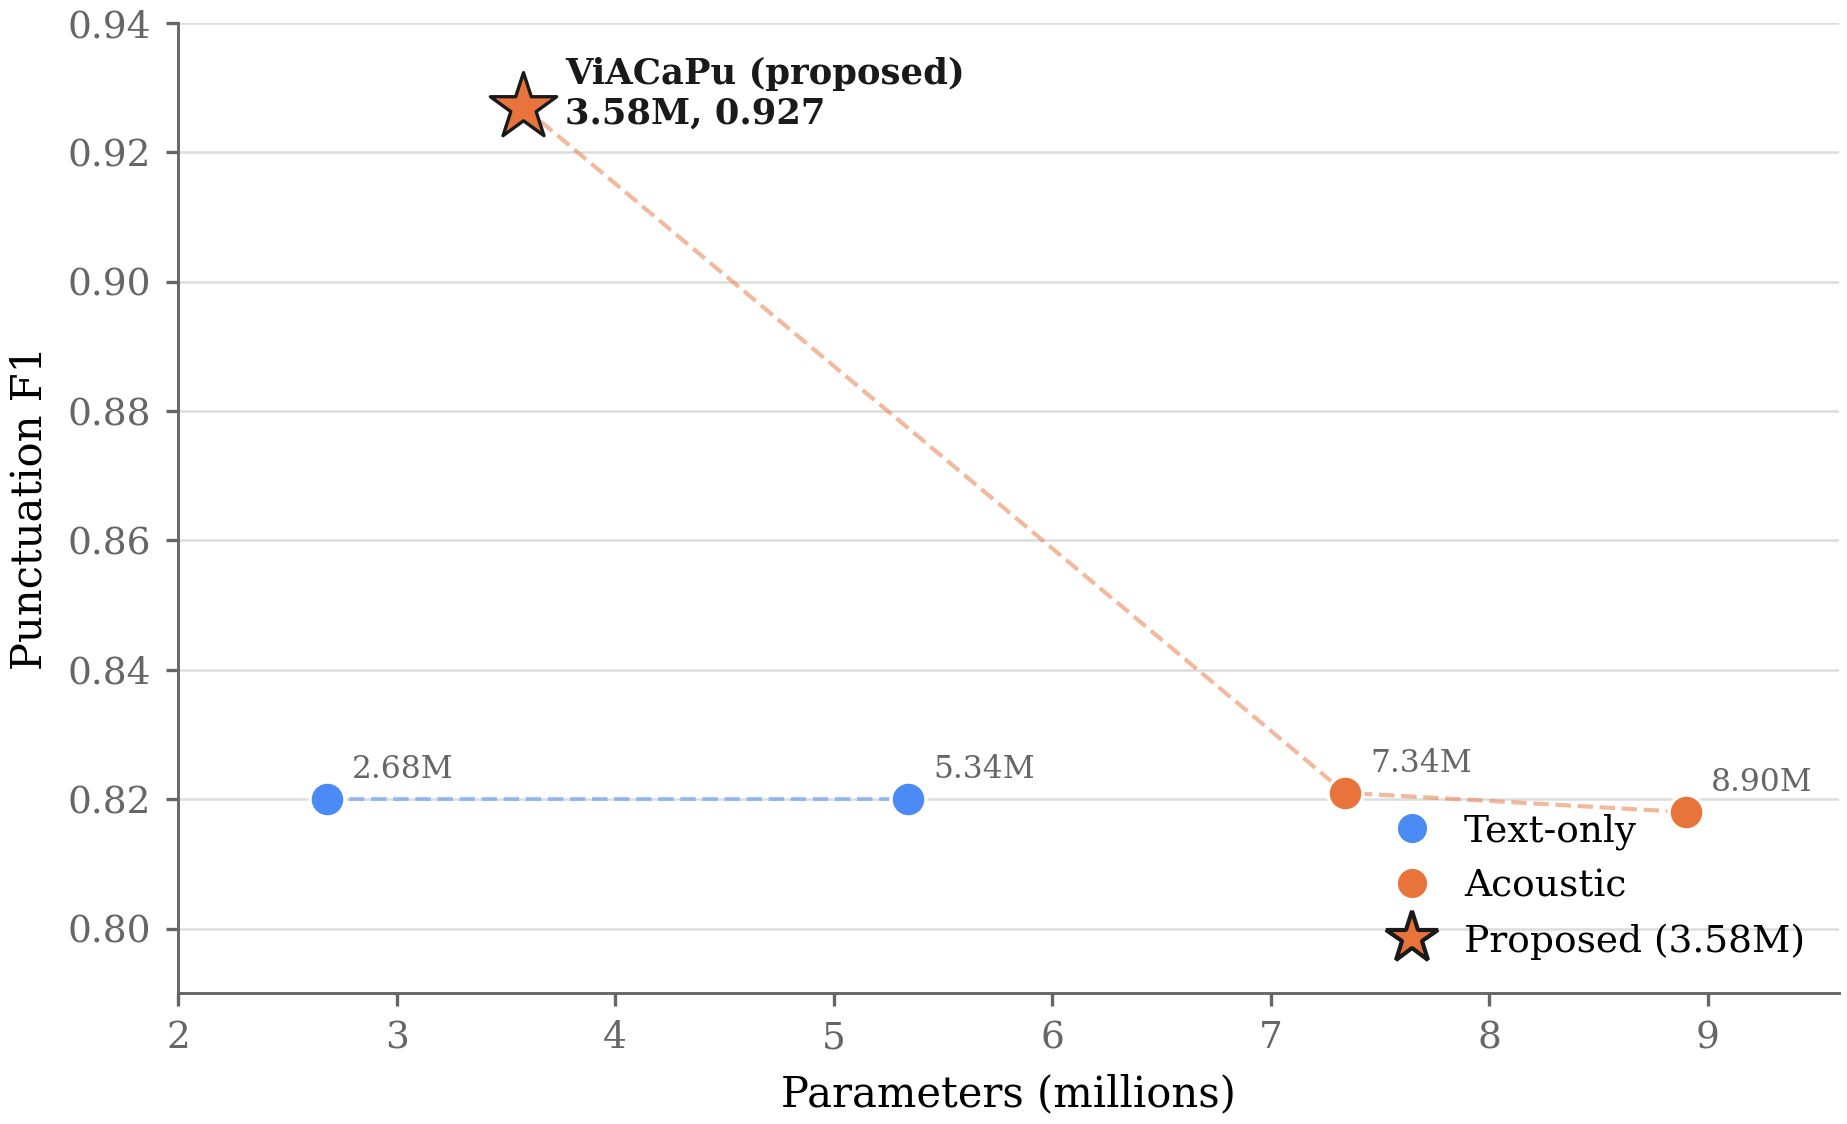
\includegraphics[width=0.72\textwidth]{figures/fig5_capacity_ablation.png}}
\caption{F1 dấu câu theo số tham số, tất cả cùng đo trên một tập kiểm định âm
thanh với cùng công thức 12 epoch. Trong các cấu hình đã thử, chất lượng không tăng
theo số tham số: mô hình 3.58M vượt các biến thể lớn hơn, còn cấu hình ngữ âm
$d{=}384$ cho kết quả gần mức text-only.}
\label{fig:ablation}
\end{figure}

Bảng~\ref{tab:ablation} và Hình~\ref{fig:ablation} cô lập ảnh hưởng của dung lượng trong khi giữ nguyên dữ
liệu, cách chia tập và công thức huấn luyện. Từ đó rút ra bốn nhận định.

Thứ nhất, khi \emph{không} có mất mát phụ, chất lượng không tăng theo số tham
số: cấu hình 3.58M (ngữ âm\,+\,aux) đạt F1 dấu câu 0.927, cao hơn hẳn các biến
thể 7.34M và 8.90M \emph{không kèm mất mát phụ}. Nhưng phép so sánh này lẫn hai
biến (bề rộng và mất mát phụ), nên tự nó không đủ để kết luận nguồn gốc lợi ích
là ngữ âm chứ không phải dung lượng --- đây chính là lý do chúng tôi bổ sung
nhận định thứ hai dưới đây.

Thứ hai, để cô lập ảnh hưởng của riêng bề rộng, chúng tôi huấn luyện thêm một
cấu hình $d{=}384$ kèm \emph{cùng} mất mát phụ ($\lambda_{\mathrm{aux}}=0{,}5$)
như cấu hình đề xuất, khác duy nhất ở bề rộng ẩn (dòng \emph{Ngữ
âm\,+\,aux, $d{=}384$} trong Bảng~\ref{tab:ablation}). Với gần gấp đôi số tham
số (7.34M so với 3.58M), cấu hình này đạt F1 dấu câu $0{,}928$ và COMMA
$0{,}888$ --- xấp xỉ \emph{giống hệt} cấu hình $d{=}256$ ($0{,}927$ và
$0{,}888$), chênh lệch $+0{,}001$ nằm trong biên độ nhiễu quan sát được giữa
các seed ở Bảng~\ref{tab:seed} ($\pm0{,}003$--$0{,}004$). Đây là phép so sánh
\emph{chỉ đổi một biến} (bề rộng, giữ nguyên mất mát phụ), nên nó ủng hộ kết
luận: một khi bộ mã hóa ngữ âm đã được giám sát bằng mất mát phụ, việc tăng gấp
đôi bề rộng ẩn không mang lại cải thiện đáng kể. Lợi ích 0.927 của cấu hình đề
xuất do đó không đến từ dung lượng lớn hơn, mà đến từ sự hiện diện của bằng
chứng ngữ âm được giám sát đúng cách. Cần lưu ý giới hạn: đối chứng $d{=}384$
này được chạy với \emph{một seed}, nên kết luận đúng ở đây là ``không quan sát
được cải thiện'' chứ không phải ``đã chứng minh không có cải thiện''; chênh lệch
$+0{,}001$ nhỏ hơn biến thiên giữa các seed nên không phân biệt được với không.

Thứ ba, các biến thể $d{=}384$ \emph{không} kèm mất mát phụ trong
Bảng~\ref{tab:ablation} cho F1 dấu phẩy ($\approx\!0.66$) gần như trùng với mô
hình chỉ dùng văn bản, tức rơi vào đúng chế độ ``ngữ âm không engage'' đã phân
tích ở Mục~\ref{sec:ablation}. Điều này nhất quán với chẩn đoán của chúng tôi:
khi thiếu tín hiệu giám sát tường minh, việc bộ mã hóa ngữ âm có học được đặc
trưng hữu ích hay không là bấp bênh, và ở các cấu hình này nó đã không học
được. Chúng tôi \emph{không} còn quy hiện tượng cho ``gate collapse'', vì giá
trị cổng đo được cho thấy cổng vẫn mở cho ngữ âm (Mục~\ref{sec:ablation}).

Thứ tư, chênh lệch chi phí huấn luyện là rõ rệt: $d{=}384$ cần khoảng
1612--1654\,s mỗi epoch (tùy có mất mát phụ hay không), so với 433--444\,s của
cấu hình $d{=}256$, tức chậm hơn khoảng $3.6$--$3.7\times$, trong khi không cho
chất lượng cao hơn (kể cả ở cấu hình có mất mát phụ). Mô hình 3.58M vì vậy đạt
điểm cân bằng tốt hơn hẳn giữa chất lượng, số tham số và chi phí huấn luyện
trong số các cấu hình đã thử.

\subsection{Ảnh hưởng của huấn luyện đúng miền}


\begin{figure}[htbp]
\centering
\centerline{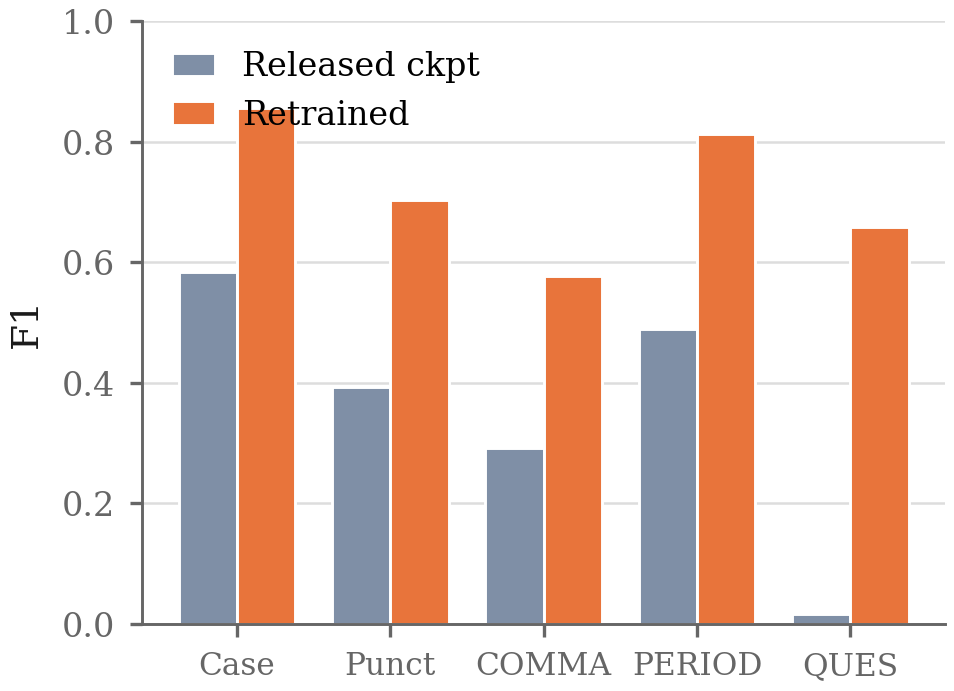
\includegraphics[width=0.72\textwidth]{figures/fig6_base_domain_shift.png}}
\caption{Checkpoint công bố của~\cite{you2024lightweight} so với cùng kiến trúc
được huấn luyện lại trên Dolly, cả hai đánh giá trên tập kiểm tra Dolly.}
\label{fig:domain}
\end{figure}

Hình~\ref{fig:domain} định lượng độ dịch miền trên tập kiểm tra gốc của mô hình cơ
sở: khi áp dụng trực tiếp cho tiếng Việt, checkpoint cơ sở công bố chỉ đạt 0.393 F1
dấu câu (QUESTION gần như không nhận ra); huấn luyện lại chính kiến trúc đó trên
Dolly nâng con số này lên 0.703. Do đó, mọi so sánh trong Bảng~\ref{tab:main} đều
dùng phiên bản đã huấn luyện lại.

Cần làm rõ vì sao cùng một checkpoint đạt $0{,}703$ trên tập này nhưng chỉ
$0{,}569$ trên tập kiểm định chung 13\,162 đoạn dùng ở Bảng~\ref{tab:main}. Hai
tập không phải cùng một dữ liệu: tập ``kiểm tra gốc'' ở đây là tập valid nội bộ
của repo cơ sở~\cite{you2024lightweight} (12\,978 đoạn tiếng Việt trích từ Dolly,
tên tệp kế thừa quy ước \texttt{IWSLT2011} từ pipeline gốc chứ không phải dữ
liệu tiếng Anh), còn tập kiểm định chung là 13\,162 đoạn được chúng tôi tách
bằng \texttt{RandomState(42)} trên toàn bộ Dolly-1000h (Bảng~\ref{tab:data}).
Chúng tôi xác nhận độ dài câu trung bình của hai tập gần như bằng nhau
($\approx$21.6 và 21.7 từ/câu) nên phần chênh lệch $0{,}703 \to 0{,}569$
\emph{không đến từ khác biệt độ dài câu}; nội dung câu của hai tập là rời nhau
(kiểm tra bằng cách đối chiếu trực tiếp không thấy trùng dòng), nhưng chúng tôi
chưa định lượng được yếu tố cụ thể nào trong 658\,128 đoạn của tập kiểm định
chung (miền chủ đề, phong cách viết, hay đơn giản là quy mô mẫu lớn hơn hẳn)
gây ra khoảng cách này. Đây là một giới hạn của phép so sánh: chúng tôi báo cáo
cả hai con số một cách minh bạch, nhưng \emph{mọi kết luận chính của bài đều
dùng con số $0{,}569$ trên tập kiểm định chung}, vì đó là tập duy nhất mà cả
ba mô hình (cơ sở, ViACaPu chỉ-văn-bản, ViACaPu\,+\,aux) được chấm cùng lúc.

\section{Thảo Luận}

\textbf{Ngôn điệu giúp ở đâu.} Phần cải thiện không đồng đều giữa các lớp mà tập
trung đúng nơi lý thuyết ngôn ngữ dự đoán. Dấu phẩy, vốn trùng với khoảng lặng
trong lời nói tự nhiên, tăng $+0.228$ F1; viết hoa, quyết định bởi manh mối từ
vựng và vị trí, gần như không đổi ($+0.007$). Sự tương phản giữa hai tác vụ này
--- cùng một mô hình, cùng một biểu diễn hợp nhất, nhưng chỉ tác vụ gắn với ngôn
điệu được hưởng lợi --- phù hợp với giả thuyết rằng nhánh ngữ âm đang khai thác
các manh mối prosody hữu ích.

Lớp QUESTION đáng lẽ cũng được hưởng lợi, vì câu hỏi được đánh dấu bởi đường ngữ
điệu lên ở cuối. Quan sát được là $0{,}733\pm0{,}014 \rightarrow 0{,}752\pm0{,}006$,
tức $+0{,}019$ --- nhưng độ lệch chuẩn giữa các seed của riêng cấu hình
chỉ-văn-bản đã là $0{,}014$, nên \emph{mức cải thiện này không tách được khỏi
nhiễu}. Với chỉ 0.25\,\% số token được chấm điểm (khoảng 34\,500 nhãn), lớp này
quá hiếm để kết luận bất cứ điều gì; chúng tôi báo cáo con số nhưng không coi
đó là bằng chứng ủng hộ giả thuyết ngôn điệu. Đồng thời, ablation dung lượng cho thấy phần cải thiện này không
thể được giải thích đơn thuần bằng việc tăng số tham số.

\textbf{Về cơ chế: bằng chứng can thiệp, không chỉ tương quan.} Khác với chỉ quan
sát ``lớp nào cải thiện'', thí nghiệm mất mát phụ ở Mục~\ref{sec:ablation} là một
\emph{can thiệp có kiểm soát}: khi ta buộc bộ mã hóa ngữ âm dự đoán năng lượng khung
(một đại lượng gắn trực tiếp với khoảng lặng/động lực tiếng nói), lợi ích ngữ âm
chuyển từ bấp bênh theo seed sang ổn định và tái lập được. Điều này xác lập chắc
chắn rằng \emph{giám sát trực tiếp bộ mã hóa ngữ âm} là thành phần quyết định.
Tuy vậy, như đã nêu ở Mục~\ref{sec:ablation}, thí nghiệm hiện tại chưa phân biệt
được giữa hai cách giải thích: mục tiêu năng lượng có tác dụng \emph{nhờ nội dung
ngôn điệu} của nó, hay đơn thuần \emph{nhờ cung cấp gradient trực tiếp và sớm}
cho một nhánh vốn chỉ nhận tín hiệu học gián tiếp. Phân biệt hai khả năng này
cần một ô đối chứng với mục tiêu phụ không mang thông tin ngôn điệu; cùng với
việc định vị chính xác từng khoảng lặng mà mô hình dựa vào (probe theo khung hoặc
can thiệp cục bộ vào pause), đây là hướng nghiên cứu tiếp theo.

\textbf{Cân bằng chi phí--lợi ích.} Nhánh ngữ âm và khối hợp nhất cộng lại thêm
0.91 triệu tham số ($+34\,\%$ tương đối), đổi lấy $+0.107$ F1 dấu câu (chênh lệch
ghép cặp theo seed). Khi tăng bề rộng lên 7.34 triệu tham số tại
$d{=}384$ --- kể cả khi giữ nguyên mất mát phụ để so sánh công bằng --- chất
lượng không tăng ($0{,}928$ so với $0{,}927$) mà chi phí \emph{huấn luyện} mỗi
epoch cao hơn khoảng $3.7\times$ (Mục~\ref{sec:capacity}). Cấu hình 3.58 triệu
tham số vì vậy là lựa chọn hợp lý trong số các cấu hình đã khảo sát. Về phía
triển khai, mô hình xuất sang ONNX và lượng tử hoá INT8 cho tệp 4.93\,MB, nhỏ
hơn mức 7\,MB của mô hình cơ sở~\cite{you2024lightweight} trong khi F1 dấu câu
cao hơn $0{,}358$ --- nghĩa là lợi ích chất lượng ở đây không đánh đổi bằng
kích thước triển khai.

\textbf{Hàm ý thiết kế.} Cơ chế hợp nhất không yêu cầu dấu thời gian mức từ:
mỗi biểu diễn từ truy vấn trực tiếp chuỗi khung ngữ âm bằng cross-attention. Điều
này giúp giảm yêu cầu căn chỉnh khi tích hợp với một hệ ASR đã có, miễn là pipeline
cung cấp văn bản nhận dạng và đoạn âm thanh hoặc đặc trưng log-Mel tương ứng. Cổng
$\mathbf{Z}$ cũng cung cấp một cơ chế học để điều chỉnh tương đối đóng góp của
luồng văn bản và ngữ âm. Tuy nhiên, khả năng hoạt động dưới nhiễu và trong pipeline
trực tuyến thực tế chưa được đánh giá riêng.

\textbf{Hạn chế.} Hạn chế đáng kể nhất nằm ở giả định về đầu vào: mọi thí nghiệm
dùng \emph{bản ghi tham chiếu} đã hạ chữ thường và bỏ dấu câu, tức tương ứng với một
bộ nhận dạng có WER bằng không. Trong pipeline thực tế, đầu vào là văn bản nhận dạng
có lỗi, và lỗi thay thế hay chèn/xóa từ có thể ảnh hưởng tới cả nhánh văn bản lẫn sự
căn chỉnh mềm giữa từ và khung âm học. Do đó các con số trong bài nên được hiểu là
\emph{chặn trên} của chất lượng khi triển khai; đánh giá trên đầu ra ASR thật ở nhiều
mức WER là bước thực nghiệm cần thiết tiếp theo. Ngoài ra, đánh giá hiện tại bao phủ
một ngôn ngữ và một miền tiếng nói;
mức độ chuyển giao của các cải thiện phụ thuộc vào việc quy ước dấu câu của bộ dữ
liệu phản ánh trung thực cách ngắt nghỉ của người nói đến đâu, thay vì theo phong
cách biên tập. Lớp QUESTION vẫn là lớp yếu nhất (F1 $0{,}746$--$0{,}756$ qua ba
seed), phản ánh sự khan hiếm của nó (0.25\,\% số vị trí được chấm, khoảng
34\,500 nhãn). Mức cải thiện $+0{,}019$ so với biến thể chỉ-văn-bản nhỏ hơn độ
lệch chuẩn giữa các seed của chính biến thể đó ($0{,}014$), nên chúng tôi
\emph{không} rút ra kết luận nào riêng cho QUESTION --- kể cả kết luận ủng hộ
giả thuyết ngôn điệu, dù lớp này về lý thuyết phải được hưởng lợi. Về mặt cơ chế, dù thí nghiệm mất mát phụ cho thấy nhánh
ngữ âm giúp \emph{nhờ} mã hóa đặc trưng năng lượng/ngôn điệu, chúng tôi chưa định vị
được chính xác từng khoảng lặng mà mô hình khai thác; đây là mức phân tích sâu hơn
để lại cho tương lai. Bộ siêu tham số còn lại (hệ số mất mát chính, trọng số lớp,
bề rộng $d$) chủ yếu được kế thừa hoặc chọn theo một tập cấu hình giới hạn, chưa qua
tìm kiếm đầy đủ, nên chưa thể tuyên bố là tối ưu; riêng trọng số mất mát phụ
$\lambda_{\mathrm{aux}}$ mới được thử ở một vài giá trị. Các kết quả chính được báo
cáo trên một tập kiểm định 2\,\% tách từ Dolly-1000h qua 3 seed; chưa có tập test
độc lập dành riêng. Với $N=3$, chúng tôi không chạy kiểm định thống kê chính thức
(ví dụ $t$-test hay Wilcoxon) vì cỡ mẫu này không đủ để suy diễn có ý nghĩa; bằng
chứng mạnh nhất mà cỡ mẫu cho phép là chênh lệch ghép cặp theo từng seed nhất quán
về dấu (Mục~\ref{sec:ablation}), và chúng tôi trình bày kết quả ở dạng
trung bình\,$\pm$\,độ lệch chuẩn thay vì tuyên bố ý nghĩa thống kê. Về khía cạnh
triển khai, lập luận về tính phù hợp với thiết bị biên trong bài dựa trên
\emph{ngân sách tham số} (3.58 triệu) và \emph{kích thước mô hình sau lượng tử
hoá}: xuất ViACaPu sang ONNX rồi lượng tử hoá động trọng số về INT8 cho tệp
\textbf{4.93\,MB} (từ 13.71\,MB ở FP32), tức nhỏ hơn $1{,}4\times$ so với mức
7\,MB mà~\cite{you2024lightweight} công bố cho mô hình cơ sở --- đây là phép so
sánh cùng đơn vị đo, vì cả hai đều là tệp ONNX đã lượng tử hoá. Cần nêu rõ ba
giới hạn của con số này. Thứ nhất, kích thước tệp không phụ thuộc phần cứng nên
so sánh được, nhưng nó \emph{không} thay thế cho các phép đo phụ thuộc phần
cứng: chúng tôi \emph{không} đo độ trễ suy luận, RTF hay bộ nhớ đỉnh trên thiết
bị biên thật. Thứ hai, chúng tôi mới xác nhận mô hình INT8 \emph{nạp và chạy
được}, chứ chưa chấm lại F1 của nó trên tập kiểm định, nên chưa loại trừ được
khả năng lượng tử hoá làm giảm chất lượng. Thứ ba, đầu phụ dự đoán năng lượng
đã được loại khỏi đồ thị xuất, đúng như thiết kế (Mục~\ref{sec:audio}).
Cuối cùng, kiến trúc hiện dùng
các lớp hai chiều (BiLSTM/BiGRU), nên chưa phải mô hình streaming theo nghĩa nhân
quả nghiêm ngặt; đánh giá chunked/causal là một hướng thực nghiệm tiếp theo.

\section{Kết Luận}
\label{sec:conclusion}

Chúng tôi đã trình bày ViACaPu, một mô hình 3.58 triệu tham số nhận biết ngữ âm cho
khôi phục dấu câu và viết hoa, hợp nhất biểu diễn văn bản và log-Mel bằng
cross-attention có cổng mà không yêu cầu dấu thời gian mức từ. Trên Dolly-1000h
tiếng Việt, mô hình đạt F1 dấu câu $0.927\pm0.004$ và F1 dấu phẩy $0.888\pm0.007$
(trung bình 3 seed), nâng F1 dấu câu $+0.107$ và dấu phẩy $+0.228$ so với biến thể
chỉ dùng văn bản cùng kiến trúc và cùng tập kiểm định, với 0.91 triệu tham số bổ
sung. Phát hiện phương pháp cốt lõi đến từ một lưới tách biến trên ba seed: khi bộ
mã hóa ngữ âm chỉ được huấn luyện gián tiếp, kết quả phân thành hai chế độ tách
biệt --- nhánh ngữ âm hoặc đóng góp đầy đủ (0.922), hoặc suy biến hoàn toàn về mức
chỉ-văn-bản (0.819--0.820) --- và trong phạm vi khảo sát, \emph{riêng} mất mát phụ
dự đoán năng lượng đã đủ để đưa cả ba seed lên 0.926\,$\pm$\,0.003, trong khi ép
cổng hợp nhất mở sớm không mang lại gì. Cơ chế đằng sau còn để ngỏ giữa hai khả
năng --- nội dung ngôn điệu của mục tiêu phụ, hay đơn thuần là việc bộ mã hóa nhận
được gradient trực tiếp --- và cần một ô đối chứng nữa để phân biệt. Ablation dung lượng, gồm một đối chứng $d{=}384$
(7.34M tham số) huấn luyện với cùng mất mát phụ, cho F1 dấu câu 0.928 --- gần
như giống hệt mức 0.927 của cấu hình 3.58M --- nên lợi ích quan sát được đến
từ bằng chứng ngữ âm được giám sát đúng cách, không phải từ số tham số lớn hơn.
Phân tích theo lớp
cho thấy cải thiện tập trung mạnh nhất ở COMMA, phù hợp với giả thuyết rằng bằng
chứng ngữ âm bổ sung các manh mối prosody hữu ích. Hướng tiếp theo là đánh giá trên
tập test độc lập, đánh giá với đầu ra ASR thật ở nhiều mức WER, định vị chính xác
các khoảng lặng mà mô hình khai thác, và nghiên cứu biến thể causal hoặc chunked
cho triển khai streaming thực sự.

\begin{thebibliography}{00}

\bibitem{you2024lightweight}
J.~You and X.~Li, ``A light-weight and efficient punctuation and word casing
prediction model for on-device streaming ASR,'' Cisco Systems, \emph{arXiv
preprint arXiv:2407.13142}, 2024.

\bibitem{unipunc}
Y.~Zhu, L.~Wu, S.~Cheng, and M.~Wang, ``Unified multimodal punctuation
restoration framework for mixed-modality corpus,'' in \emph{Proc. IEEE ICASSP},
2022.

\bibitem{stpt}
A.~Jakubiak \emph{et al.}, ``Adapting ASR models for speech-to-punctuated-text
recognition with utterance gluing,'' Samsung R\&D Institute Poland, in
\emph{Proc. ICNLSP}, 2025.

\bibitem{jointcappunc}
H.~T.~T. Uyen, N.~A. Tu, and T.~D. Huy, ``Vietnamese capitalization and
punctuation recovery models,'' in \emph{Proc. INTERSPEECH}, 2022.

\bibitem{cho2022}
J.~Y. Cho, S.~Ng, T.~Tran, and M.~Ostendorf, ``Leveraging prosody for punctuation
prediction of spontaneous speech,'' in \emph{Proc. INTERSPEECH}, 2022.

\bibitem{che2020}
X.~Che \emph{et al.}, ``Multimodal semi-supervised learning framework for
punctuation prediction in conversational speech,'' \emph{arXiv preprint
arXiv:2008.00702}, 2020.

\bibitem{bertpunct}
A.~Nagy, B.~Bial, and J.~\'Acs, ``Automatic punctuation restoration with BERT
models,'' \emph{arXiv preprint arXiv:2101.07343}, 2021.

\bibitem{survey}
V.~P\u{a}i\c{s} and D.~Tufi\c{s}, ``Capitalization and punctuation restoration:
a survey,'' \emph{Artificial Intelligence Review}, 2022.

\bibitem{polacek2023}
M.~Pol\'a\v{c}ek \emph{et al.}, ``Online punctuation restoration using ELECTRA
model for streaming ASR systems,'' in \emph{Proc. INTERSPEECH}, 2023.

\bibitem{lightweight2025}
M.~Pol\'a\v{c}ek \emph{et al.}, ``Lightweight online punctuation and
capitalization restoration for streaming ASR systems,'' \emph{Speech
Communication}, vol.~173, 2025.

\bibitem{kim2023}
J.~Kim \emph{et al.}, ``Improved training for end-to-end streaming automatic
speech recognition model with punctuation,'' in \emph{Proc. INTERSPEECH}, 2023.

\bibitem{librispeechpc}
A.~Meister \emph{et al.}, ``LibriSpeech-PC: Benchmark for evaluation of
punctuation and capitalization capabilities of end-to-end ASR models,'' in
\emph{Proc. IEEE ASRU}, 2023.

\bibitem{nguyen2019}
B.~Nguyen \emph{et al.}, ``Fast and accurate capitalization and punctuation for
automatic speech recognition using transformer and chunk merging,'' in
\emph{Proc. O-COCOSDA}, 2019.

\bibitem{sunkara2020}
M.~Sunkara \emph{et al.}, ``Robust prediction of punctuation and truecasing for
medical ASR,'' in \emph{Proc. ACL Workshop on NLP for Medical Conversations},
2020.

\bibitem{trinh2026}
T.~T.~H. Trinh, N.~H. Tran, D.~T. Nguyen, V.~H. Hoang, T.~V. La, N.~H. Pham, and
N.~Mai Xuan, ``End-to-end Vietnamese ASR with acoustic-aware punctuation and
capitalization for edge devices,'' \emph{J. Sci. Technol. --- Smart Systems and
Devices}, vol.~36, 2026.

\bibitem{whisper}
A.~Radford \emph{et al.}, ``Robust speech recognition via large-scale weak
supervision,'' in \emph{Proc. ICML}, 2023; \emph{large-v3-turbo} variant
(809M parameters), OpenAI, 2024.

\end{thebibliography}

%% ================== GHI CHÚ TIẾNG VIỆT ==================
%% Nếu \usepackage[utf8]{vietnam} báo lỗi (không có gói `vietnam`), thay bằng:
%%    \usepackage[T5]{fontenc}\usepackage[utf8]{inputenc}
%%    \usepackage[vietnamese]{babel}
%% Hoặc dùng XeLaTeX/LuaLaTeX với:
%%    \usepackage{fontspec}\usepackage{polyglossia}\setmainlanguage{vietnamese}
%% Trên Overleaf: Menu -> Compiler -> pdfLaTeX (mặc định) thường đã có gói `vietnam`.
\end{document}